\documentclass[a4paper, 12pt, fleqn]{report}
\usepackage[utf8]{vietnam}
\usepackage{amsmath}
\usepackage{setspace}
\setstretch{1.2}
\usepackage{geometry}
\usepackage{tocbibind}
\usepackage[toc,page]{appendix}
\usepackage{multirow}
\usepackage{longtable}
\usepackage{acronym}

\usepackage{tabularx}
\usepackage{graphicx}
\usepackage[export]{adjustbox}

\usepackage{caption}
\usepackage{subcaption}
\usepackage{float}
\setlength\parindent{0pt}
\usepackage[ruled]{algorithm2e}

\usepackage {fancybox} 

\usepackage{tikz}
\usetikzlibrary{calc}

\usepackage{algpseudocode}
% \usepackage{algpascal}
% \usepackage{algorithmicx}


\usepackage{mathtools}
\DeclarePairedDelimiter\floor{\lfloor}{\rfloor}


\usepackage{scrextend}
\changefontsizes{13pt}

\usepackage{sectsty}
\chaptertitlefont{\LARGE}

\geometry{
    top = 20mm,
    bottom = 20mm,
    left = 35mm,
    right = 25mm
}
% \author{Sinh viên: Nguyễn Duy Mạnh}

% \title{ĐỒ ÁN TỐT NGHIỆP}

\begin{document}
% \maketitle

\begin{titlepage}
    \begin{tikzpicture}[remember picture, overlay]
        \draw[line width = 2pt] ($(current page.north west) + (1in,-1in)$) rectangle ($(current page.south east) + (-0.5in,0.5in)$);
      \end{tikzpicture}

    \begin{center}
        % \vspace*{1cm}

        \textbf{TRƯỜNG ĐẠI HỌC BÁCH KHOA HÀ NỘI}\\
        \textbf{VIỆN CÔNG NGHỆ THÔNG TIN VÀ TRUYỀN THÔNG}\\
        \_\_\_\_\_\_\_\_\_\_\_\_\_\_\_\_\_\_\_\_\_\_\_\_\
        \vspace*{1cm}

        \includegraphics[width=0.2\textwidth]{picture/bklogo.jpg}
        \vspace*{1cm}
  
        \LARGE
        \textbf{ĐỒ ÁN}

        \Huge
        \textbf{TỐT NGHIỆP ĐẠI HỌC}
        
        \large
        \textbf{NGÀNH CÔNG NGHỆ THÔNG TIN}
        
        
        \vspace{1cm}
        \large
        \textbf{Các thuật toán metaheuristics trong bài toán tối ưu tuổi thọ mạng cảm biến không dây}
  
        \vspace{1.5cm}
  
        \begin{table}[H]
            \raggedleft
            \begin{tabular}{rl}
            \textbf{Sinh viên thực hiện:} & Nguyễn Duy Mạnh               \\
                                 & Lớp CNTT2.2 - K59             \\
            \textbf{Giáo viên hướng dẫn:} & PGS. TS. Huỳnh Thị Thanh Bình \\
                                 & ThS. Nguyễn Thị Tâm          
            \end{tabular}
        \end{table}
  
        \vfill
  
        
  
        \vspace{0.8cm}
  
       
  
        
        HÀ NỘI 05-2019
  
    \end{center}
\end{titlepage}


\pagenumbering{gobble}
\begin{center}
    \textbf{PHIẾU GIAO NHIỆM VỤ ĐỒ ÁN TỐT NGHIỆP}
\end{center}

\textbf{1. Thông tin sinh viên}
\\Họ và tên: NGUYỄN DUY MẠNH 
\\Lớp: CNTT2.2 - K59 \qquad\qquad\qquad\qquad\qquad{ }{} Hệ đào tạo: Đại học chính quy 
\\Điện thoại liên lạc: 0975713207 \qquad Email: nguyenduymanhbk59@gmail.com 
\\Đồ án tốt nghiệp được thực hiện tại: bộ môn Khoa học máy tính, viện Công nghệ thông tin và truyền thông, trường Đại học Bách Khoa Hà Nội
\\Thời gian làm đồ án tốt nghiệp: từ ngày 12/01/2019 đến ngày 23/05/2019

\textbf{2. Mục đích nội dung của ĐATN}
\begin{itemize}
    \item Tìm hiểu bài toán tối ưu tuổi thọ mạng cảm biến không dây 
    \item Đề xuất giải thuật metaheuristic giải bài toán tối ưu tuổi thọ mạng cảm biến không dây 
\end{itemize}

\textbf{3. Các nhiệm vụ cụ thể của ĐATN}
\begin{itemize}
    \item Tìm hiểu bài toán tối ưu tuổi thọ mạng cảm biến không dây 
    \item Đề xuất giải thuật metaheuristic giải bài toán tối ưu tuổi thọ mạng cảm biến không dây 
    \item Tiến hành cài đặt các giải thuật đề xuất 
    \item Thực nghiệm, so sánh, đánh giá kết quả 
\end{itemize}

\textbf{4. Lời cam đoan của sinh viên}
\\Tôi – Nguyễn Duy Mạnh - cam kết ĐATN là công trình nghiên cứu của bản thân tôi dưới sự hướng dẫn của PGS.TS. Huỳnh Thị Thanh Bình và ThS. Nguyễn Thị Tâm. Các kết quả nêu trong ĐATN là trung thực, không phải là sao chép toàn văn của bất kỳ công trình nào khác.
\begin{table}[H]
    \raggedleft
    \begin{tabular}{c}
    \textit{Hà Nội, ngày 23 tháng 05  năm 2019} \\
    Tác giả ĐATN                                \\
                                                \\
    \textit{Nguyễn Duy Mạnh}                   
    \end{tabular}
\end{table}

\textbf{5. Xác nhận của giáo viên hướng dẫn về mức độ hoàn thành của ĐATN và cho phép bảo vệ}
\begin{table}[H]
    \raggedleft
    \begin{tabular}{c}
    \textit{Hà Nội, ngày\qquad tháng \qquad năm 2019} \\
    Giáo viên hướng dẫn                          \\
                                                \\
    \textit{Huỳnh Thị Thanh Bình}               
    \end{tabular}
\end{table}
\chapter*{Tóm tắt đồ án}
Hiện nay, mạng cảm biến không dây đang phát triển cực kì mạnh mẽ và được áp dụng vào hàng loạt lĩnh vực khác nhau. Song hành cùng với sự phát triển là thách thức, trong đó năng lượng cũng như thời gian mạng hoạt động là một vấn đề then chốt. Đồ án này tập trung vào vấn đề tuổi thọ của mạng cảm biến không dây, nhiều mô hình của bài toán này đã được đưa ra trong các nghiên cứu, nhận thấy rằng có thể cải thiện một số điểm để sát với thực tế, đồ án đã đưa ra một mô hình mới cũng như đề xuất cách giải quyết cho mô hình.

Nội dung của đồ án gồm 5 chương:

\textit{Chương 1} trình bày tổng quan các khái niệm của bài toán tối ưu cùng các phương pháp chính xác và xấp xỉ để  giải quyết bài toán, giải thuật di truyền và một số khái niệm cơ bản trong lý thuyết đồ thị.

\textit{Chương 2} giới thiệu bài toán tối ưu thời gian sống của mạng cảm biến không dây cùng các nghiên cứu liên quan, sau đó đưa ra mô hình đề xuất.

\textit{Chương 3} đề xuất giải thuật di truyền giải bài toán tối ưu tuổi thọ mạng cảm biến không dây.

\textit{Chương 4} đề xuất phương pháp giải quyết bài toán bằng cách kết hợp tìm kiếm cục bộ kết hợp và giải bài toán luồng cực đại trong mạng.

\textit{Chương 5} trình bày về thực nghiệm, nhận xét và đánh giá các đề xuất.
% \include{abstract_of_thesis}
% \include{loi_noi_dau}
\chapter*{Lời cảm ơn}
Lời đầu tiên, em xin gửi lời cảm ơn chân thành nhất đến các thầy giáo, cô giáo bộ môn Khoa học máy tính nói riêng, viện Công nghệ Thông Tin và Truyền Thông cũng như các thầy cô của trường đại học Bách Khoa Hà Nội đã truyền thụ cho em những kiến thức quý báu trong suốt năm 5 học tập tại trường. Đồng thời em cũng xin gửi lời cảm ơn đặc biệt đến PGS. TS. Huỳnh Thị Thanh Bình, cô không chỉ truyền thụ kiến thức mà còn hướng dẫn, chỉ dạy những kĩ năng, kinh nghiệm quý báu, giúp em có thêm những hành trang cho chặng đường tiếp theo khi bước ra cổng trường đại học.
\BlankLine
Xin cảm ơn ThS. Nguyễn Thị Tâm cùng các bạn, các em trong nhóm nghiên cứu phòng thí nghiệm Mô hình hóa, mô phỏng và tối ưu hóa trường Đại học Bách Khoa Hà Nội, cảm ơn mọi người đã cùng tìm tòi, chia sẻ giúp em mở rộng, nâng cao kiến thức.
\BlankLine
Cảm ơn gia đình đã luôn là động lực to lớn, là chỗ dựa vững chắc nhất những khi khó khăn, giúp con không nản lòng mà phấn đấu vươn lên.

\begin{table}[H]
    \raggedleft
    \begin{tabular}{c}
    \textit{Hà Nội, ngày  23  tháng   05   năm 2019} \\
                                                     \\
    \textit{Nguyễn Duy Mạnh}                        
    \end{tabular}
\end{table}

\tableofcontents

\listoffigures
\listoftables
\chapter*{Danh mục từ viết tắt}
\addcontentsline{toc}{chapter}{Danh mục từ viết tắt}

\begin{table}[H]
    \begin{tabularx}{\linewidth}{|l|X|X|}
    \hline
    \multicolumn{1}{|c|}{\textbf{Từ viết tắt}} & \multicolumn{1}{c|}{\textbf{Viết đầy đủ}} & \multicolumn{1}{c|}{\textbf{Ý nghĩa}}             \\ \hline
    WSN                                       & Wireless Sensor Network       & Mạng cảm biến không dây                                        \\ \hline
    WUSN                                       & Wireless Underground Sensor Network       & Mạng cảm biến không dây ngầm                      \\ \hline
    GA                                         & Genetic Algorithm                         & Giải thuật di truyền                              \\ \hline
    GAH                                        & Genetic Algorithm with Heuristic          & Giải thuật di truyền kết hợp thuật toán heuristic \\ \hline
    LSMF                                       & Local Search with Max Flow                & Tìm kiếm cục bộ kết hợp thuật toán luồng cực đại  \\ \hline
    \end{tabularx}
\end{table}

\pagenumbering{arabic} 
\setcounter{page}{1}
\chapter{Cơ sở lí thuyết}
\section{Bài toán tối ưu}
Trong thực tế, ta thường gặp những vấn đề có nhiều cách giải quyết, một cách tự nhiên ta chọn cách giải quyết vấn đề một cách tối ưu nhất, chẳng hạn như nhanh nhất, tốn ít thời gian nhất hay mang lại hiệu quả kinh tế cao nhất... Đó được gọi là những bài toán tối ưu hóa.

Trong khoa học máy tính, bài toán tối ưu là bài toán tìm ra lời giải “tốt” nhất trong các lời giải khả thi. Tùy vào bài toán khác nhau sẽ định nghĩa độ tốt khác nhau, thường được gọi chung là hàm mục tiêu của bài toán. Có nhiều cách để phân chia lớp các bài toán tối ưu, một cách thường gặp là dựa vào tính chất của biến trong bài toán để chia bài toán thành hai loại: 
\begin{itemize}
    \item Bài toán tối ưu hóa liên tục: biến trong bài toán là biến liên tục. 
    \item Bài toán tối ưu hóa rời rạc (hay còn gọi là tối ưu hóa tổ hợp): biến trong bài toán là biến rời rạc.
\end{itemize}
Phần sau trình bày về hai dạng bài toán tối ưu trên. 

\subsection{Tối ưu hóa liên tục}
Theo \cite{convex_optimization}, dạng tiêu chuẩn của bài toán tối ưu hóa liên tục 
\[\begin{array}{lll}
    \mbox{minimize} & f(x)\\
    \mbox{subject to} & g_i(x) \leq 0 & i = 1, 2, ..., m\\
    \mbox{} & h_i(x) = 0 & i = 1, 2, ..., p\end{array}\]
Trong đó:
\begin{itemize}
    \item $f(x): R^n \rightarrow R$ là hàm mục tiêu cần đạt được 
    \item $g_i(x) \leq$ 0 được gọi là các ràng buộc bất đẳng thức 
    \item $h_i(x)$ = 0 là các ràng buộc đẳng thức 
    \item $m, p \in N$
\end{itemize}
Theo quy ước, dạng tiêu chuẩn xác định một bài toán cực tiểu hóa. Ta có thể định nghĩa bài toán cực đại hóa một cách tương tự.
\\Một ví dụ thường gặp của bài toán tối ưu liên tục là tối ưu giá trị của hàm số trong đoạn/khoảng cho trước.
\begin{figure}[H]
    \centering
    \includegraphics[width=0.8\linewidth]{picture/continuous_func.png}
    \caption{Đồ thị hàm $f(x) = x * sin(10\pi * x) + 1$}
\end{figure}
\subsection{Tối ưu hóa tổ hợp}
Như đã nêu ở trên, bài toán tối ưu tổ hợp là bài toán có biến quyết định nhận các giá trị rời rạc. Một cách tổng quát, một bài toán tối ưu tổ hợp có thể được định nghĩa bởi bộ ba ($S$, $f$, $\Omega$), trong đó $S$ là tập hữu hạn trạng thái (lời giải tiềm năng hay phương án), $f$ là hàm mục tiêu xác định trên $S$, $\Omega$ là tập các ràng buộc. Mỗi lời giải $s\in S$ thỏa mãn $\Omega$ được gọi là một lời giải chấp nhận được. Mục tiêu ở đây là tìm phương án $s^*$ tối ưu hóa toàn cục hạm mục tiêu $f$. Chẳng hạn với bài toán cực tiểu hóa thì $f(s^*) \leq f(s)$ với mọi phương án chấp nhận được $s$.
\\Ta đi đến một số bài toán tiêu biểu của lớp các bài toán tối ưu hóa tổ hợp. 
\\ \\\textbf{Bài toán người du lịch}
\\Nội dung bài toán: một người du lịch muốn tham quan $n$ thành phố $T_1, T_2, …, T_n$. Xuất phát từ một thành phố bất kì, người du lịch muốn đến tất cả các thành phố còn lại, mỗi thành phố đi qua đúng một lần rồi quay trở lại thành phố xuất phát. Gọi $C_{ij}$ là chi phí đi từ thành phố $T_i$ đến thành phố $T_j$, hãy tìm một hành trình thõa mản yêu cầu bài toán sao cho tổng chi phí di chuyển là nhỏ nhất.
\\Bài toán được mô hình hóa như sau 
\\Đầu vào:
\begin{itemize}
    \item $n$: số thành phố 
    \item $C_{nxn}$: ma trận kích thước n x n trong đó $c_{ij}$ là chi phí di chuyển từ thành phố i đến thành phố j
\end{itemize}
Đầu ra:
\begin{itemize}
    \item Hành trình đi qua n thành phố $T_{\pi(1)}, T_{\pi(2)}, …, T_{\pi(n)}$
\end{itemize}
Mục tiêu: tối thiểu hóa chi phí di chuyển  
\begin{equation}
    f = C_{\pi(1),\pi(2)}, C_{\pi(2),\pi(3)}, …, C_{\pi(n),\pi(1)} \rightarrow min
\end{equation}
Ràng buộc: mỗi thành phố chỉ đi qua một lần 
\begin{equation}
    \pi(i) \neq \pi(j) ~\forall ~1 \leq i, j \leq n
\end{equation}
Một cách lí thuyết, bài toán người du lịch sẽ có tất cả $n^n$ lời giải, tuy nhiên sẽ chỉ có $n!$ lời giải hợp lệ do ràng buộc mỗi thành phố chỉ được phép đi qua một lần. Nhiệm vụ tối ưu là tìm lời giải có tổng chi phí di chuyển nhỏ nhất trong $n!$ lời giải hợp lệ.
\\ \\\textbf{Bài toán cái túi}
\\Nội dung bài toán: một nhà thám hiểm cần đem theo một cái túi có trọng lượng không quá $b$. Có $n$ đồ vật có thể đem theo, đồ vật thứ $i$ có trọng lượng $a_i$ và giá trị sử dụng $c_i$ ($i$ = 1, 2, …, $n$). Hỏi nhà thám hiểm cần đem theo những đồ vật nào để tổng giá trị sử dụng là lớn nhất.

Một phương án của nhà thám hiểm có thể biểu diễn bởi một vector nhị phân có độ dài $n$: $z$ = ($z_1$, $z_2$, …, $z_n$), trong đó $z_i$ = 1 có nghĩa đồ vật thứ $i$ được mang theo và bằng 0 nếu ngược lại. 
\\Tổng giá trị các đồ vật đem theo là:
\begin{equation}
    f(x) = \sum_{i=1}^{n}c_ix_i
\end{equation}
Tổng trọng lượng đồ vật đem theo là:
\begin{equation}
    g(x) = \sum_{i=1}^{n}a_ix_i
\end{equation}
Đầu vào:
\begin{itemize}
    \item $n$ đồ vật 
    \item $b$ là trọng lượng tối đa có thể mang theo 
    \item $a = (a_1, a_2, ..., a_n): a_i$ là trọng lượng của vật $i$
    \item $c = (c_1, c_2, ..., c_n): c_i$ là trọng lượng của vật $i$
\end{itemize}
Đầu ra: 
\begin{itemize}
    \item Biến nhị phân $z = (z_1, z_2, ..., z_n): z_i$ = 1 khi vật $i$ được chọn 
\end{itemize}
Hàm mục tiêu: 
\begin{equation}
        f(x) = \sum_{i=1}^{n}c_ix_i \rightarrow max 
\end{equation}
Ràng buộc:
\begin{equation}
        g(x) = \sum_{i=1}^{n}a_ix_i \leq b 
    \end{equation}
\section{Các phương pháp giải bài toán tối ưu}
Giải bài toán tối ưu chính là đi tìm đáp án tốt nhất trong hàng loạt các đáp án khả thi của không gian lời giải. Có thể thu được lời giải tối ưu hàm mục tiêu trong không gian này nhưng đôi khi ta cũng chỉ có thể thu được lời giải “được coi là” tốt, liên quan đến hai khái niệm sau
\begin{itemize}
	\item Tối ưu toàn cục: lời giải tốt nhất thu được trong không gian lời giải của bài toán.
	\item Tối ưu cục bộ: lời giải tốt nhất trong một tập con của không gian lời giải.
\end{itemize}
Vậy vì sao lại dẫn đến trường hợp chỉ có kết quả “được coi là” tốt (tối ưu cục bộ)? Ta điểm qua các phương pháp giải bài toán tối ưu để làm rõ vấn đề này.
\subsection{Các phương pháp giải chính xác}
Như tên gọi, phương pháp giải chính xác cho bài toán tối ưu là phương pháp đem lại lời giải tốt nhất trong toàn bộ không gian lời giải của bài toán. Tiêu biểu là một số phương pháp sau.
\\ \\\textbf{Vét cạn}
\\Vét cạn là kĩ thuật với ý tưởng rất đơn giản: thử tất cả các phương án có thể của bài toán, kiểm tra liệu lời giải có vi phạm ràng buộc, kết luận phương án nào là tối ưu.
\\Phương pháp này có thể đảm bảo lời giải được tìm ra là tối ưu do đã xét mọi trường hợp có thể xảy ra, tuy nhiên lại gặp một trở ngại rất lớn: thời gian. Xét với một ví dụ đơn giản là bài toán người du lịch đã nêu ở trên, tập các lời giải khả thi là n!, chỉ cần tăng thêm một thành phố vào bài toán thì số lời giải khả thi đã tăng theo cấp số nhân, do đó phương pháp vét cạn hiển nhiên không thể áp dụng để giải bài toán này một cách hiệu quả.
\\ \\\textbf{Nhánh cận}
\\Ý tưởng của phương pháp nhánh cận đó là nếu ta dự đoán trước được những phương án có hàm mục tiêu chắc chắn tồi hơn hàm mục tiêu của phương án đã có trước đó, vậy ta không cần thử qua những phương án này nữa, nhờ đó thu hẹp được không gian tìm kiếm. Đây là một cải tiến của phương pháp vét cạn, cho phép tìm ra được lời giải nhanh hơn.
\\Trong phương pháp nhánh cận, ta sẽ xây dựng từng phần của lời giải cho đến khi tìm ra được lời giải tối ưu. Mô hình hóa lời giải thành vector $x = (x_1, x_2, …, x_n)$, giả sử tại bước $k$ ta đã xây dựng được $k$ thành phần của lời giải từ $x_1$ đến $x_k$, cần mở rộng thành phần $x_{k+1}$, nhưng khi đánh giá lại ta thấy tất cả các nghiệm mở rộng từ $x_k$ không có nghiệm nào có giá trị tốt hơn giá trị tối ưu ta đã biết tại thời điểm đó, vậy ta không cần mở rộng nữa, như vậy ta đã cắt bỏ đi một nhánh. 
\\Điều khó là phải đánh giá được các thành phần mở rộng, nếu đánh giá được tốt, thuật toán nhánh cận sẽ chạy nhanh hơn nhiều so với vét cạn. Tuy nhiên nhánh cận vẫn chỉ có thể áp dụng trong các bài toán có quy mô nhỏ.
\\ \\\textbf{Chia để trị}
\\Chia để trị là một phương pháp áp dụng cho các bài toán có thể giải quyết bằng cách chia nhỏ ra thành các bài toán con từ việc giải quyết các bài toán này. Sau đó lời giải của bài toán nhỏ được tổng hợp lại thành lời giải cho bài toán ban đầu.
Kĩ thuật chia để trị là cơ sở cho nhiều thuật toán hiệu quả, chẳng hạn như thuật toán sắp xếp, thuật toán nhân, thuật toán phân tích cú pháp. 
\\Kĩ thuật chia để trị thông qua ba bước:
\begin{itemize}
    \item Chia/tách nhỏ: tại bước này bài toán ban đầu được tách thành các bài toán con cho đến khi không thể tách được nữa, các bài toán con sẽ trở thành một bước nhỏ trong việc giải quyết bài toán lớn.
    \item Trị/giải quyết bài toán con: tại bước này sẽ tìm cách giải quyết bài toán con một cách cụ thể.
    \item Tổng hợp: khi đã giải quyết được các bài toán con, tổng hợp lại để có được lời giải của bài toán ban đầu.
\end{itemize}
\textbf{Quy hoạch động}
\\Được nhà toán học Richard Bellman phát minh vào năm 1953, quy hoạch động là một phương pháp mạnh mẽ tìm lời giải chính xác của các bài toán tối ưu. Phương pháp này thường dùng để giải các bài toán có cấu trúc con tối ưu và bài toán có các bài toán con gối nhau \cite{gtvlt}.
\\ \emph{Bài toán con gối nhau}, tương tự như chia để trị, quy hoạch động cũng chia bài toán ban đầu thành các bài toán con nhỏ hơn. Quy hoạch động được sử dụng khi các bài toán con này gọi đi gọi lại, kết quả của các bài toán con được lưu lại, do đó giảm thời gian tính toán.
Quy hoạch động sẽ không thể áp dụng được khi các bài toán con không gối nhau, do mỗi lần chia nhỏ, mỗi bài toán con chỉ được gọi một lần mà không được gọi lại.
\\ \emph{Cấu trúc con tối ưu} có nghĩa là các lời giải tối ưu cho các bài toán con có thể được sử dụng để tìm các lời giải tối ưu cho bài toán toàn cục. Ví dụ, đường đi ngắn nhất tới một đỉnh trong một đồ thị có thể được tìm thấy bằng cách: trước hết tính đường đi ngắn nhất tới đích từ tất cả các đỉnh kề nó, rồi dùng kết quả này để chọn đường đi toàn cục tốt nhất. Nói chung, ta có thể giải một bài toán với cấu trúc con tối ưu bằng một quy trình ba bước:
\begin{itemize}
    \item Chia bài toán thành các bài toán con nhỏ hơn.
    \item Giải các bài toán này một cách tối ưu bằng cách sử dụng đệ quy quy trình ba bước này.
    \item Sử dụng các kết quả tối ưu đó để xây dựng một lời giải tối ưu cho bài toán ban đầu.
\end{itemize}
Các bài toán con được giải bằng cách chia chúng thành các bài toán con nhỏ hơn, và cứ tiếp tục như thế cho đến khi ta đến được trường hợp đơn giản dễ tìm lời giải.
\\Quy hoạch động thường dùng thường dùng hai cách tiếp cận:
\begin{itemize}
    \item Top-down (từ trên xuống): chia bài toán ban đầu thành các bài toán con, giải và ghi nhớ lại lời giải của các bài toán con này phòng khi cần dùng. Đây là đệ quy và lưu trữ kết hợp với nhau.
    \item Bottom-up (từ dưới lên): tất cả các bài toán con có thể cần đến đều được giải trước, sau đó được dùng để xây dựng lời giải cho bài toán lớn hơn. Cách tiếp cận này tốt hơn về không gian bộ nhớ dùng cho ngăn xếp và số lời gọi hàm. 
\end{itemize}
Trên đây đã điểm qua một số phương pháp giải chính xác cho bài toán tối ưu hóa. Tuy nhiên đôi khi không thể tìm ra phương pháp giải chính xác cho bài toán tối ưu ngoại trừ vét cạn, hoặc có thể tìm được nhưng không gian lời giải bùng nổ cực kì nhanh khi kích thước bài toán tăng lên. Trong trường hợp đó sẽ cần sử dụng các phương pháp giải xấp xỉ để giải quyết bài toán.
\subsection{Các phương pháp giải xấp xỉ}
Đến nay đã có rất nhiều phương pháp giải xấp xỉ được đề xuất để giải quyết các bài toán tối ưu khác nhau. Dưới đây là một số ví dụ tiêu biểu.
\\ \\\textbf{Thuật toán tham lam }
\\Thuật toán tham lam giải quyết bài toán theo hướng luôn chọn tối ưu địa phương tại mỗi bước đi với hy vọng tìm được lời giải tối ưu toàn cục. Ví dụ với bài toán người du lịch, tại mỗi bước ta sẽ chọn thành phố tiếp theo bằng cách chọn thành phố gần nhất chưa đi qua.
Nói chung, thuật toán tham lam bao gồm năm phần:
\begin{itemize}
    \item Tập hợp các ứng viên để tạo ra lời giải. 
    \item Một hàm lựa chọn để theo đó chọn ứng viên tốt nhất để bổ sung vào lời giải.
    \item Một hàm khả thi, theo đó quyết định một ứng viên có phù hợp để đưa vào lời giải.
    \item Hàm mục tiêu, xác định giá trị của lời giải.
    \item Hàm đánh giá, chỉ ra khi nào lời giải hoàn chỉnh.
\end{itemize}
Giải thuật tham lam quyết định sớm hướng đi và không bao giờ xét lại các quyết định cũ. Đối với một số bài toán, đây có thể là một thuật toán không chính xác.
\\ \\\textbf{Tìm kiếm cục bộ}
\\Kĩ thuật tìm kiếm cục bộ đưa ra lời giải bằng cách tại mỗi bước cố gắng di chuyển đến lời giải láng giềng của lời giải hiện tại sao cho hàm mục tiêu được cải thiện. Các bước của kĩ thuật này như sau:
\begin{itemize}
    \item Xuất phát từ một lời giải bất kì. 
    \item Áp dụng một phép biến đổi lên lời giải hiện hành để thu được một lời giải tốt hơn. 
    \item Lặp lại phép biến đổi lên phương án hiện tại cho đến khi không thể cải thiện được nữa.
\end{itemize}
Do một phép biến đổi thường chỉ làm thay đổi một phần của phương án hiện tại để được một phương án mới nên được gọi là biến đổi địa phương, vì thế kĩ thuật này có tên tìm kiếm cục bộ.
\\ \\\textbf{Các thuật toán tiến hóa }
\\Thuật toán tiến hóa là tên gọi chung để chỉ lớp các thuật toán tìm kiếm và tối ưu hóa dựa trên nguyên lý tiến hóa tự nhiên. Một số thuật toán tiến hóa đã được công bố \cite{lap_trinh_tien_hoa}:
\begin{itemize}
    \item Quy hoạch tiến hóa: do D.B.Pogel đề xuất. Có thể diễn tả quy hoạch tiến hóa như sau: cho một lớp các phương pháp khả dĩ giải quyết được một (số) phần của vấn đề. Dựa vào quy luật tiến hóa, tìm một phương pháp liên hợp đủ khả năng giải quyết trọn vẹn vấn đề đó.
    \item Chiến lược tiến hóa: do T.Baeck, F.H.Hofmeister và H.P.Schwefel đề xuất. Thuật toán này dựa trên một số chiến lược ban đầu, tiến hóa để tạo ra những chiến lược mới phù hợp với môi trường thực tế một cách tốt nhất.
    \item Giải thuật di truyền: do J.H.Holland đề xuất, được D.E.Goldberg, L.Davis và Z.Michalevicz phát triển. Dựa trên quan niệm cho rằng quá trình tiến hóa tự nhiên là quá trình hoàn hảo nhất, hợp lý nhất và tự nó đã mang tính tối ưu \cite{lap_trinh_tien_hoa}.
\end{itemize}
Tiến hóa tự nhiên là một quá trình tối ưu. Đây có thể xem như một mệnh đề đúng, không chứng minh được, nhưng phù hợp với thực tế khách quan \cite{lap_trinh_tien_hoa}. Quá trình tiến hóa thể hiện tính tối ưu ở chỗ: thế hệ sau bao giờ cũng tốt hơn (phát triển hơn, hoàn thiện hơn) thế hệ trước. Tiến hóa tự nhiên được duy trì nhờ vào hai quá trình cơ bản: sinh sản và chọn lọc tự nhiên. Xuyên suốt quá trình tiến hóa tự nhiên, các thế hệ mới luôn được sinh ra để bổ sung thay thế thế hệ cũ. Cá thể nào phát triển hơn, thích ứng tốt hơn với môi trường sẽ tồn tại, ngược lại sẽ bị đào thải. Sự thay đổi môi trường là động lực thúc đẩy quá trình tiến hóa, đồng thời quá trình tiến hóa cũng làm thay đổi môi trường.
\\Các cá thể mới sinh ra nhờ sự lai ghép ở thế hệ cha mẹ. Một cá thể mới có thể mang các đặc tính của cha mẹ (di truyền) nhưng cũng có thể mang các đặc tính hoàn toàn khác (đột biến). Di truyền và đột biến có vai trò quan trọng như nhau trong quá trình tiến hóa, dù rằng đột biến xảy ra với xác suất nhỏ hơn nhiều so với di truyền. Các thuật toán tiến hóa tuy có những điểm khác biệt nhưng đều mô phỏng các quá trình cơ bản: lai ghép, đột biến, chọn lọc.
\begin{itemize}
    \item Lai ghép: là quá trình sinh ra cá thể mới bằng cách thừa hưởng các đặc tính từ cá thể cha mẹ.
    \item Đột biến: là hiện tượng cá thể con sinh ra mang một số tính trạng không có trong mã di truyền của cha mẹ.
    \item Chọn lọc: dựa trên cơ sở độ thích nghi của các cá thể, chọn ra các cá thể tốt phù hợp với môi trường.
\end{itemize}
\section{Giải thuật di truyền}
Giải thuật di truyền \cite{lap_trinh_tien_hoa} xuất hiện lần đầu vào năm 1962 trong công trình nghiên cứu về các hệ thống thích ứng của John Henry Holland, sau này được tiếp tục phát triển bởi chính học trò của ông là nhà khoa học David Edward Goldberg. Đến năm 1975, giải thuật di truyền chính thực được trình bày trong cuốn sách Adaptation in Natural and Artificial Systems (Thích nghi trong tự nhiên và trong các hệ thống nhân tạo).
\\Thuật giải di truyền sử dụng các thuật ngữ vay mượn của di truyền học. Ta có thể nói về các cá thể (hay kiểu gen, cấu trúc) trong một quần thể, những cá thể này có thể được gọi là chuỗi (hay nhiễm sắc thể). Điều này có thể gây lẫn lộn: mỗi tế bào của một cơ thể chủng loại đã cho mang một số những nhiễm sắc thể nào đó nhưng trong thuật giải di truyền, ta chỉ nói về những cá thể có một nhiễm sắc thể. Các nhiễm sắc thể được tạo thành từ các đơn vị (các gen) – biểu diễn trong một chuỗi tuyến tính. Mỗi gen kiểm soát một số đặc trưng.
\\Mỗi nhiễm sắc thể biểu diễn một lời giải của bài toán đang giải, một tiến trình tiến hóa được thực hiện trên một quần thể các các nhiễm sắc thể tương ứng với một quá trình tìm kiếm lời giải trong không gian lời giải. Tìm kiếm đó cần cân đối hai mục tiêu (có vẻ mâu thuẫn nhau): khai thác những lời giải tốt nhất và khảo sát không gian tìm kiếm, điểm mạnh của giải thuật di truyền là duy trì và xử lý một tập các lời giải (quần thể) trong suốt quá trình tìm kiếm, tạo được sự cân đối đáng kể giữa hai yêu tố trên. Nhờ việc duy trì nhiều lời giải này, giải thuật di truyền tìm kiếm trên nhiều điểm song song có khả năng leo lên nhiều cực trị cùng một lúc. Thông qua các toán tử của mình, giải thuật trao đổi thông tin giữa các cực trị với nhau, từ đó làm giảm thiểu khả năng giải thuật kết thúc tại các cực trị địa phương và bỏ qua mất cực trị toàn cục.
\\Tiếp theo đi vào chi tiết các bước của giải thuật di truyền.
\subsection{Mã hóa cá thể}
Công việc đầu tiên cần thực hiện khi giải bài toán bằng giải thuật di truyền là chọn cách biểu diễn cá thể. Mã hóa cá thể là việc ánh xạ các tham số của bài toán lên một chuỗi có chiều dài xác định, tùy theo từng bài toán cụ thể mà có các cách biêu diễn khác nhau sao cho phù hợp, thuận lợi khi giải toán. Đây là công việc cực kì quan trọng, một cách biểu diễn mã hóa cá thể tốt quyết định tới 50\% thành công của giải thuật.
\\Có nhiều cách mã hóa cá thể nhưng có hai cách biểu diễn thông dụng nhất là biểu diễn nhị phân và biểu diễn sử dụng hoán vị.
Với biểu diễn nhị phân, mỗi cá thể tương ứng với một chuỗi bao gồm các bit 0 và 1, ý nghĩa của các bit này phụ thuộc vào từng tính huống cụ thể. Đây là cách biểu diễn đơn giản và thông dụng nhất trong các cách biểu diễn.
\\Ví dụ trong bài toán cái túi được nêu ở trên, có một cách mã hóa cá thể đơn giản như sau: đánh thứ tự $n$ đồ vật từ 1 đến $n$, mỗi cá thể được biểu diễn bằng một xâu nhị phân độ dài $n$, bit thứ $i$ bằng 1 có nghĩa là đồ vật thứ $i$ được chọn cho vào túi và bằng 0 nếu ngược lại.
Trong biểu diễn hoán vị, mỗi cá thể tương ứng với một hoán vị của tập $n$ ký hiệu nào đó. Chẳng hạn với bài toán người du lịch đã được nêu ở trên, với $n$ thành phố, ký hiệu cho các thành phố lần lượt là $T_1, T_2, …, T_n$. Mỗi cá thể, sự mã hóa của lời giải sẽ là một danh sách hoán vị của $T_1, T_2, …, T_n$ biểu diễn lộ trình mà người du lịch đã đi qua. 
\subsection{Khởi tạo quần thể }
Như đã nêu ở trên, giải thuật di truyền duy trì và xử lí một tập các lời giải trong suốt quá trình tìm kiếm, khởi tại quần thể chính là quá trình sinh ra các cá thể một số lượng nhất định (kích thước quần thể).
\\Quần thể được khởi tạo ban đầu sẽ ảnh hưởng tới tốc độ của giải thuật và đôi khi là cả kết quả cuối cùng, vì vậy việc khởi tạo các cá thể ban đầu của quần thể cũng cần sử dụng phương pháp phù hợp với bài toán. Có hai cách khởi tạo thường gặp là khởi tạo ngẫu nhiên và khởi tạo heuristic.
\begin{itemize}
    \item Khởi tạo ngẫu nhiên: cá thể được sinh ra một cách ngẫu nhiên, miễn là đáp ứng được các ràng buộc của bài toán.
    \item Khởi tạo heuristic: dựa vào các kinh nghiệm đã có, ta khởi tạo tập các cá thể với hi vọng tập này có một khởi đầu tốt hơn nhằm nhanh chóng tìm ra lời giải.    
\end{itemize}
\subsection{Các toán tử di truyền }
Các phép lai ghép, đột biến được gọi chung là các toán tử di truyền, các toán tử này sẽ quyết định chiều hướng tiến hóa của quần thể, do đó để đảm bảo kết quả tốt, ta cần có các toán tử lai ghép và đột biến phù hợp.
\subsubsection{Lai ghép}
Quá trình lai ghép diễn ra bằng cách ghép một hay nhiều đoạn gen từ hai nhiễm sắc thể cha-mẹ để hình thành nhiễm sắc thể mới mang đặc tính cả cha lẫn mẹ. Các cá thể mới thừa hưởng các đặc tính tốt sẽ có khả năng sinh tồn mạnh hơn, nhờ đó duy trì nguồn gen tốt trong quần thể.
\\Một số phép lai ghép cơ bản: lai ghép một điểm cắt, lai ghép hai điểm cắt.
Trong lai ghép một điểm cắt, một điểm phân cách được chọn ra, khi đó phần nằm phía sau điểm phân cách này của hai cá thể cha mẹ được hoán đổi với nhau sinh ra hai con mới. Tương tự với phép lai ghép hai điểm cắt, có hai điểm phân cách được chọn, phần tráo đổi là phần nằm giữa hai điểm cắt. 
\\Tuy nhiên hai phép lai ghép trên phần lớn được áp dụng khi cách mã hóa cá thể là mã hóa nhị phân, với cách mã hóa cá thể khác (ví dụ mã hóa hoán vị), cá thể con sinh ra chưa chắc là một cá thể hợp lệ và do đó phép lai ghép coi như vô nghĩa. Trong trường hợp này cần áp dụng một số phép lai ghép khéo léo hơn.
\subsubsection{Đột biến}
Khác với đặc điểm của phép lai ghép là tận dụng nguồn gen tốt sẵn có trong quần thể, đột biến là quá trình tiến hóa khi một hoặc một số gen của cá thể con không được thừa hưởng từ gen của cha mẹ. Phép đột biến xảy ra với xác suất thấp hơn nhiều so với phép lai và có thể được mô tả như sau: 
\begin{itemize}
    \item Chọn ngẫu nhiên một cá thể trong quần thể.
    \item Giả sử độ dài mã hóa của cá thể là $n$, chọn một số $k$ ngẫu nhiên thỏa mãn $1 \leq k \leq n$, thay đổi gen thứ $k$ sao cho cá thể vẫn phù hợp.
    \item Trả cá thể này về quần thể để tham gia quá trình tiến hóa tiếp theo.
\end{itemize}
\subsection{Hàm thích nghi }
Hàm thích nghi phản ánh độ tương thích của cá thể với môi trường, hàm thích nghi có giá trị càng tốt chứng tỏ cá thể càng mạnh, là đối tượng phù hợp để giữ lại trong quá trình tiến hóa.
\\Có nhiều cách chọn hàm thích nghi khác nhau tùy vào bài toán, một cách chọn hàm thích nghi phổ biến là sử dụng luôn hàm mục tiêu trong mô hình bài toán đã đề ra.
\subsection{Chọn lọc}
Chọn lọc là quá trình loại bỏ các cá thể xấu và để lại những cá thể tốt. Một số phương pháp chọn lọc phổ biến như: 
\begin{itemize}
    \item Sắp xếp quần thể theo độ thích nghi, chỉ giữ lại các cá thể tốt nhất.
    \item Chọn lọc theo bánh xa Roullette: các cá thể được xếp vào một vòng tròn với độ rộng của cung tương ứng với độ thích nghi, quay vòng tròn bằng cách sinh ra một số ngẫu nhiên trong khoảng (0, 1) rồi chọn ra cá thể tương ứng.
\end{itemize}
\subsection{Điều kiện dừng của giải thuật}
Điều kiện được đưa ra để đảm bảo tính dừng của giải thuật. Thường giải thuật di truyền dừng lại sau một số thế hệ xác định hoặc dừng khi sau một số thế hệ không cải thiện được hàm mục tiêu của bài toán. Đây là một tham số của bài toán sẽ được chọn ra một cách phù hợp trong quá trình thực nghiệm.
\subsection{Đánh giá giải thuật di truyền}
Ưu điểm:
\begin{itemize}
    \item Nhanh hơn và tốn ít tài nguyên hơn so với tìm kiếm truyền thống trong một không gian tìm kiếm lớn.
    \item Đơn giản, nếu có cách mã hóa cá thể chuẩn xác và hàm mục tiêu đúng, ta có thể tìm được lời giải mà không cần thực hiện quá nhiều công việc phức tạp.
\end{itemize}
Nhược điểm: 
\begin{itemize}
    \item Đây không phải là một giải thuật hoàn chỉnh do không phải lúc nào giải thuật cũng tìm được lời giải phù hợp.
    \item Có thể bị mắc tại các cục bộ địa phương, mặc dù phép đột biến có thể giúp giảm thiểu trường hợp này nhưng làm giải thuật tiêu tốn nhiều thời gian hơn.
    \item Đôi khi khó để tìm được cách mã hóa cá thể.    
\end{itemize}
\section{Lý thuyết đồ thị}
\subsection{Các khái niệm cơ bản về đồ thị}
Lý thuyết đồ thị là một lĩnh vực nghiên cứu đã có từ lâu đời và có nhiều ứng dụng trong thế giới hiện đại. Những tư tưởng cơ bản của lý thuyết đồ thị được đề xuất vào những năm đầu của thế kỷ 18 bởi nhà toán học lỗi lạc người Thụy sỹ - Leonhard Euler. Chính ông là người đã sử dụng đồ thị để giải bài toán nổi tiếng về 7 cây cầu ở thành phố Konigsberg.
\\Đồ thị là cấu trúc rời rạc có tính trực quan cao, rất tiện ích để biểu diễn các quan hệ. Có thể kể đến một số ứng dụng thực tế của đồ thị như:
\begin{itemize}
    \item Có tiềm năng trong nhiều lĩnh vực do đồ thị có thể dùng để biểu diễn mối quan hệ, nghiên cứu quan hệ giữa các đối tượng là mục tiêu của nhiều lĩnh vực khác nhau.
    \item Ứng dụng trong mạng máy tính, mạng giao thông, mạng cung cấp nước, mạng điện, lập lịch, tối ưu hóa hệ thống, thiết kế mạch, quy hoạch phát triển,…
    \item Các ứng dụng khác: phân tích gen, trò chơi máy tính, chương trình dịch, thiết kế hướng đối tượng,…
\end{itemize}
Sau đây sẽ trình bày các khái niệm của đồ thị, nền tảng cho việc áp dụng lí thuyết đồ thị để giải quyết bài toán kéo dài thời gian sống của mạng cảm biến.
\subsection{Định nghĩa đồ thị}
Đồ thị là một tập các đối tượng được gọi là đỉnh, nối với nhau bởi các cạnh. Các loại đồ thị khác nhau được phân biệt bởi kiểu và số lượng cạnh nối. Ta định nghĩa các loại đồ thị như sau:

Đơn (đa) đồ thị vô hướng $G = (V, E)$ là cặp gồm 
\begin{itemize}
    \item Tập đỉnh $V$ là tập hữu hạn phần tử, các phần tử gọi là đỉnh 
    \item Tập cạnh $E$ là tập các bộ không có thứ tự dạng $(u, v), u, v \in E, u \neq v$
\end{itemize}
Đơn (đa) đồ thị có hướng $G = (V, E)$ là cặp gồm 
\begin{itemize}
    \item Tập đỉnh $V$ là tập hữu hạn phần tử, các phần tử gọi là đỉnh 
    \item Tập $E$ là tập các bộ có thứ tự dạng $(u, v), u, v \in E, u \neq v    $
\end{itemize}
\subsection{Đường đi và chu trình}
Định nghĩa: đường đi P độ dài n từ đỉnh u đến đỉnh v, trong đó n là nguyên dương, trên đồ thị $G = (V, E)$ là dãy
\begin{itemize}
    \item $P: x_0, x_1, …, x_n$
    \item Trong đó $u = x_0, v = x_n, (x_i, x_{i+1}) \in E, i = 0, 1, 2, …, n-1$
    \item Đỉnh $u$ gọi là đỉnh đầu, đỉnh $v$ gọi là đỉnh cuối của đường đi
\end{itemize}
Đường đi nói trên còn có thể biểu diễn dưới dạng dãy các cạnh: $(x_0, x_1)$, $(x_1, x_2)$, …, $(x_{n-1}, x_n)$.
\\Đường đi gọi là đường đi đơn nếu không có đỉnh nào bị lặp lại trên nó.
\\Đường đi gọi là đường đi cơ bản nếu không có cạnh nào bị lặp lại trên nó.
\\Nếu có đường đi từ đỉnh $u$ đến đỉnh $v$ thì ta nói đỉnh $v$ đạt đến được từ đỉnh $u$. Ta quan niệm rằng đỉnh v luôn đạt đến được từ chính nó.
\\Định nghĩa: đường đi cơ bản có đỉnh đầu trùng với đỉnh cuối ($u = v$) được gọi là chu trình.
Chu trình được gọi là đơn nếu như ngoại trừ đỉnh đầu và đỉnh cuối không có đỉnh nào bị lặp lại.
\section{Bài toán luồng cực đại }
\subsection{Các khái niệm}
Khái niệm mạng: mạng là đồ thị có hướng $G = (V, E)$
\begin{itemize}
    \item Có duy nhấtmột đỉnh $s$ không có cung đi vào gọi là đỉnh phát (nguồn) và duy nhất một đỉnh $t$ không có cung đi ra gọi là đỉnh thu (đích)
    \item Mỗi cung $e$ của $G$ được gắn với một số không âm $c(e)$ được gọi là khả năng thông qua của e
\end{itemize}
Luồng trong mạng: luồng $f$ trong mạng $G = (V, E)$ là phép gán số $f(e)$ cho mỗi cạnh $e$ ($f(e)$ được gọi là luồng trên cạnh $e$) thỏa mãn các điều kiện
\begin{enumerate}
    \item Hạn chế về khả năng thông qua 
    \begin{itemize}
        \item Với mỗi cung $e, 0 \leq f(e) \leq c(e)$
    \end{itemize}
    \item Điều kiện cân bằng luồng: với mỗi $v \neq s, t$
    \begin{itemize}
        \item $\sum_{e \in E^-(v)} f(e) = \sum_{e \in E^+(v)} f(e)$
    \end{itemize}
\end{enumerate}
Định nghĩa: giá trị của luồng $f$ là
\begin{itemize}
    \item $val(f) = \sum_{e \in E^-(s)} f(e) = \sum_{e \in E^+(t)} f(e)$
\end{itemize}
Định nghĩa: luồng trong mạng G được gọi là luồng cực đại nếu trong số tất cả các luồng trong mạng G
nó là luồng có giá trị lớn nhất. Bài toán tìm luồng cực đại trong mạng G được gọi là bài toán luồng cực
đại.
\\Định nghĩa: lát cắt là cách phân hoạch tập đỉnh $(S, T)$ sao cho $s \in S, t \in T$.
\\Khả năng thông qua $caps(S, T)$ của lát cắt $(S, T)$ là số:
\begin{itemize}
    \item $caps(S, T) = \sum_{e \in S \rightarrow T} c(e)$
    \item Trong đó: $S \rightarrow T := \{(v, w \in E: v \in S, w \in T)\}$
\end{itemize}
Lát cắt nhỏ nhất (hẹp nhất) là lát cắt với khả năng thông qua nhỏ nhất.
\\Bổ đề: giả sử $f$ là luồng, và $(S, T)$ là lát cắt. Khi đó giá trị luồng chảy qua lát cắt chính bằng giá trị luồng
\begin{itemize}
    \item $\sum_{e \in S \rightarrow T} f(e) - \sum_{e \in T \rightarrow S} f(e) = \sum_{e \in E^+(s)} f(e) = val(f)$
    \item Trong đó $S \rightarrow T := \{(v, w \in E: v \in S, w \in T)\}$ và $T \rightarrow S := \{(v, w \in E: v \in T, w \in S)\}$
\end{itemize}
Bổ đề: giả sử $f$ là luồng, còn $(S, T)$ là lát cắt, khi đó $val(f) \leq caps(S, T)$
Hệ quả: giả sử $f$ là luồng, còn $(S, T)$ là lát cắt. Nếu $val(f) = cap(S, T)$ thì $f$ là luồng cực đại, còn $(S, T)$ là lát cắt hẹp nhất.
\subsection{Định lý Ford - Fulkerson và thuật toán giải bài toán luồng cực đại}
Định lý Ford - Fulkerson: trong mạng bất kỳ, giá trị luồng cực đại luôn bằng khả năng thông qua của lát cắt nhỏ nhất.
\\ \textbf{Thuật toán Ford - Fulkerson:} 
\\Sau mỗi bước của thuật toán, các điều kiện sau cần được duy trì
\begin{itemize}
    \item $f(u, v) \leq c(u, v)$: luồng từ $u$ tới $v$ không vượt quá khả năng thông qua
    \item $f(u, v) = -f(v, u)$: ta duy trì cân bằng luồng 
    \item $\sum_f(u,v) = 0$: cho tất cả các nút ngoại trừ s và t. Lượng đi vào vào một nút bằng lượng đi ra khỏi nút đó. 
\end{itemize}
Điều này có nghĩa là một luồng đi qua mạng là một luồng hợp lệ sau mỗi bước lặp của thuật toán. Ta định nghĩa mạng thặng dư $G_f (V, E_f)$ là mạng với sức chứa $c_f (u, v) = c (u, v) - f (u, v)$ và luồng bằng không.

\begin{algorithm}[H]
    \SetKwData{START}{start}
    \SetKwData{MID}{mid}
    \SetKwData{END}{end}
    \SetKwData{Up}{up}
    \SetKwData{Energy}{E'}
    \SetKwData{ivar}{i}
    \SetKwData{jvar}{j}
    \SetKwData{TRUE}{True}
    \SetKwData{FALSE}{False}
    \SetKwData{varlone}{$l_1$}
    \SetKwData{varltwo}{$l_2$}
    \SetKwData{varlthree}{$l_3$}
    \SetKwFunction{MaxFlow}{MaxFlow}
    \SetKwFunction{FindConnect}{FindConnect}
    \SetKwInOut{Input}{Đầu vào}
    \SetKwInOut{Output}{Đầu ra}
    \Input{\\ Đồ thị $G = (V, E)$ với khả năng thông qua $c (u, v)$ \\Điểm phát s \\ Điểm thu t}
    \Output{\\Luồng $f$ từ $s$ đến $t$ sao cho $f$ có giá trị cực đại}
        \SetAlgoLined
        \BlankLine
        \Begin{
            $f(u, v) \leftarrow 0 ~\forall ~u, v$\\
            \While{tồn tại đường đi từ $s$ đến $t$ trong $G$}{
                Tìm một đường đi $u_1 , u_2 ,..., u_k$ với $u_1 = s, u_k = t$ sao cho $c_f (u_i , u_{i+1}) > 0$ \\
                Tìm $m = min (c_f (u_i , u_{i+1}))$ \\
                $f (u_i , u_{i+1}) \leftarrow f (u_i , u_{i+1} ) + m$ \\
                $f (u_{i+1} , u_i ) \leftarrow f (u_{i+1} , u_i ) - m$
            }
            \DecMargin{1em}
        }
        \caption{Thuật toán Ford - Fulkerson}      
\end{algorithm}
Đường đi trong $G_f (V, E_f)$ có thể tìm được bằng thuật toán tìm kiếm theo chiều rộng (breadth first search - BFS) hoặc tìm kiếm theo chiều sâu (depth first search – DFS).
\chapter{Bài toán tối ưu thời gian sống của mạng cảm biến không dây}

\section{Tổng quan về mạng cảm biến không dây}

\begin{figure}[h]
    \includegraphics[width=\linewidth]{picture/wsn.jpg}
    \caption{Mạng cảm biến không dây}
    \label{fig:pic1}
\end{figure}
Mạng cảm biến không dây (Wireless Sensor Network - WSN) là mạng liên
kết các nút cảm biến (sensor nodes) với nhau nhờ các liên kết không dây như sóng vô tuyến, hồng ngoại. Các thiết bị cảm biến thường đơn giản, nhỏ gọn, giá thành rẻ và phân bố rộng khắp trong khu vực cảm biến, sử dụng những nguồn năng lượng giới hạn như pin hay ắcquy. Dữ liệu sau khi thu thập được sẽ được gửi đến các trạm cơ sở (Base Stations) trực tiếp hay gián tiếp thông qua một điểm thu phát (Sinks) hoặc các điểm chuyển tiếp (relay nodes) và môi trường mạng công cộng như Internet hay vệ tinh. 
\\Các nút cảm biến không dây có thể được triển khai cho nhiều mục đích chuyên dụng với quy mô khác nhau: giám sát và điều khiển công nghiệp, tự động hóa gia đình và điện dân dụng, quân sự, y tế và giám sát sức khỏe, môi trường và nông nghiệp,... Lợi thế chủ yếu của chúng là có thể triển khai trong rất nhiều môi trường khác nhau, kể cả trong các môi trường nguy hiểm (nhiễm độc, phóng xạ,…) mà mạng có dây truyền thống không thể thực hiện được.
\\ \\\textbf{Cấu trúc của mạng cảm biến không dây}
\\Một mạng cảm biến không dây bao gồm lượng lớn các nút được triển khai dày đặc bên trong khu vực cần thu thập dữ liệu. Vị trí các cảm biến không cần định trước vì vậy nó cho phép triển khai ngẫu nhiên trong các vùng không thể tiếp cận hoặc các khu vực nguy hiểm.
Mỗi nút cảm biến được phát tán trong mạng có khả năng thu thập thông số liệu, định tuyến, số liệu về bộ thu nhận (sink) để chuyển tới người dùng và định tuyến các bản tin mang theo yêu cầu từ nút sink đến các nút cảm biến
\\Mỗi nút cảm biến gồm bốn thành phần cơ bản: bộ cảm biến, bộ xử lý, bộ thu phát sóng không dây và nguồn điện. Tùy theo ứng dụng cụ thể, nút cảm biến còn có thể có các thành phần bổ sung như hệ thống tìm vị trí, bộ sinh năng lượng và thiết bị di động. Bộ cảm biến thường gồm hai đơn vị thành phần là đầu đo cảm biến (sensor) và bộ chuyển đổi tương tự/số (ADC). Bộ xử lý thường kết hợp với một bộ nhớ nhỏ, phân tích thông tin cảm biến và quản lý các thủ tục cộng tác với các nút khác. Bộ thu phát đảm bảo thông tin giữa nút cảm biến và mạng bằng kết nối không dây. Một thành phần quan trọng của nút cảm biến là bộ nguồn, có thể là pin hoặc ắcquy, cung cấp năng lượng cho cảm biến và không thay thế được nên nguồn năng lượng của nút thường là giới hạn. Bộ nguồn có thể được hỗ trợ bởi các thiết bị sinh điện, ví dụ như các tấm pin mặt trời nhỏ.
\\ \\\textbf{Một số đặc điểm của mạng cảm biến không dây}
\\Ưu điểm
\begin{itemize}
    \item Kích thước vật lý nhỏ gọn.
    \item Hoạt động đồng thời với độ tập trung cao.
    \item Dễ dàng triển khai, mở rộng.
    \item Chi phí các thiết bị cảm biến không cao.
    \item Tính đa dạng trong thiết kế và sử dụng.
    \item Hoạt động tin cậy.
\end{itemize}
Nhược điểm
\begin{itemize}
    \item Khả năng liên kết vật lý và phân cấp điều khiển hạn chế.
    \item Thiết bị cảm biến có khả năng tính toán, lưu trữ và nguồn năng lượng hạn chế.
    \item Dư thừa dữ liệu.
    \item Truyền thông không dây dẫn tới một số vấn đề như độ ổn định, mất mát thông tin, bảo mật.
\end{itemize}
\section{Bài toán tối ưu thời gian sống của mạng cảm biến không dây }
Với sự phát triển mạnh mẽ của mình, mạng cảm biến không dây được ứng dụng vào rất nhiều lĩnh vực khác nhau như nông nghiệp, quân sự, y tế… Và để sử dụng một cách hiệu quả, rất nhiều vấn đề trong mạng cảm biến không dây được quan tâm nghiên cứu như hiệu suất, độ bao phủ, cấu trúc mạng, phương thức định tuyến… trong đó có một trong các yếu tố quan trọng bậc nhất đó là vấn đề năng lượng hay nói cách khác là thời gian sống (tuổi thọ) của mạng cảm biến, do một mạng cảm biến chỉ thực thi đầy đủ chức năng của mình khi nó còn “sống”. Cho đến nay có nhiều cách định nghĩa về tuổi thọ của mạng cảm biến không dây khác nhau do nhiều tác giả đưa ra. Ta sẽ đề cập một số cách định nghĩa phổ biến sau.
\subsection{Tuổi thọ của mạng dựa vào số nút còn hoạt động}
Cách định nghĩa phổ biến trong các tài liệu đó là $n-of-n$, trong đó tuổi thọ của mạng được định nghĩa bằng tuổi thọ của nút cảm biến có thời gian sống ít nhất.
\[T_n^n = \min_{v \in V} T_v\]
Trong đó $T_n$ là thời gian sống của nút $v$.
\\$T_n^n$ là cách định nghĩa đơn giản và thuận tiện cho tính toán, các thuật toán dùng trong mạng không cần quan tâm đến bất kì sự thay đổi nào của kiểu hình mạng. Tuy nhiên trong phần lớn trường hợp, cách định nghĩa này có ý nghĩa lớn trong các bài toán lí thuyết hơn là các ứng dụng thực tế của mạng cảm biến. Ví dụ, xét một nút cảm biến có nhiều nút hàng xóm với công năng cảm biến tương đương, nhiều mạng cảm biến hoàn toàn có thể chấp nhận được việc nút này dừng hoạt động và sử dụng các nút hàng xóm, nhưng  không xét đến các trường hợp như vậy và cho rằng mạng đã “chết”. Do đó, ta nên sử dụng cách định nghĩa này khi các nút trong mạng có độ quan trọng xấp xỉ nhau.
\\Ngoài ra còn có một số biến thể khác của $T_n^n$. Tuổi thọ của mạng được định nghĩa là thời gian nhỏ nhất của một nút từ khi bắt đầu hoạt động cho đến khi năng lượng của nút xuống thấp hơn một mức $\beta$ cho trước, hoặc cũng có thể được định nghĩa mạng còn sống khi ít nhất $k$ nút trong mạng còn hoạt động ($k-of-n - T_n^k$).
\subsection{Tuổi thọ của mạng dựa vào độ bao phủ của các nút cảm biến}
Trong khi đánh giá tuổi thọ của mạng cảm biến dựa vào số nút cảm biến còn hoạt động là một cách định nghĩa khá tổng quát thì việc xét đến các đặc điểm của mạng cảm biến, cụ thể như đánh giá tuổi thọ của mạng dựa vào độ bao phủ của các nút cảm biến với môi trường đang khảo sát có vẻ như là một cách tự nhiên hơn để định nghĩa tuổi thọ của mạng.
\\Các mô hình bao phủ trong mạng cảm biến có thể chia thành ba loại chính:
\begin{itemize}
    \item Bao phủ diện tích: mỗi điểm trong không gian khảo sát đều phải nằm trong vùng cảm biến.
    \item Bao phủ đối tượng: một số điểm định trước trong không gian phải nằm trong vùng cảm biến.
    \item Bao phủ barrier: mạng cảm biến cần có chức năng phát hiện đối tượng di chuyển vào hoặc băng qua khu vực được giám sát.
\end{itemize}
Có hai cách để mô tả độ bao phủ của một mạng cảm biến:
\begin{itemize}
    \item Một số phần trăm $\alpha$ của không gian được bao phủ bởi ít nhất một cảm biến, thường được gọi là $\alpha-coverage$.
    \item Mỗi điểm trong không gian cần được bao phủ bởi ít nhất k sensor, thường được gọi là $k-coverage$.
\end{itemize}
Nhiều nghiên cứu định nghĩa tuổi thọ của mạng dựa trên các biến thể của cách định nghĩa trên, trong đó phổ biến nhất là 1-coverage, tức là tuổi thọ của mạng được tính từ lúc bắt đầu triển khai cho đến khi tất cả các điểm cần thiết nằm trong vùng cảm biến của ít nhất một nút cảm biến.
\\Độ bao phủ thường là một yếu tố cực kì quan trọng để đánh giá hiệu quả của mạng cảm biến, tuy nhiên đánh giá tuổi thọ của mạng chỉ dựa trên độ bao phủ thì không hợp lí, do không thể đảm bảo dữ liệu thu thập được chắc chắn truyền về nút sink.
\subsection{Tuổi thọ của mạng dựa trên kết nối }
\cite{Baydere2005} và \cite{Yu2001} định nghĩa tuổi thọ của mạng dựa trên tổng số lượng gói tin có thể truyền tới nút sink. Mặc dù số lượng này có thể đóng vai trò là chỉ số cho sự bền bì của mạng, nhưng nó phụ thuộc rất nhiều vào các thuật toán cụ thể được áp dụng trong mạng. Giả sử ta áp dụng thuật toán tập hợp thông tin trong mạng, như vậy số gói tin truyền về nút sink sẽ giảm trong khi lượng thông tin nhận được vẫn là tương đương. Do đó khả năng áp dụng định nghĩa này trong việc so sánh tuổi thọ của các thiết lập mạng khác nhau sẽ bị hạn chế.
\\Một nhược điểm khác của cách định nghĩa này là số các gói tin được truyền về không phản ánh được mạng cảm biến hoạt động bình thường trong bao lâu (tính theo đơn vị thời gian).
\\Trong \cite{Giridhar} định nghĩa tuổi thọ của mạng dựa theo số lần thu thập dữ liệu từ môi trường thành công, trong đó với mỗi lần thu thập dữ liệu thì không có nút nào hết năng lượng. Cách định nghĩa này có thể quy dẫn về $T_n^n$ đã nêu ở trên, chỉ khác đó là tuổi thọ không được tính theo đơn vị thời gian mà là số lần thu thập dữ liệu.
\subsection{Tuổi thọ của mạng dựa trên độ bao phủ của các nút cảm biến và kết nối}
Do một số hạn chế của việc đánh giá tuổi thọ mạng dựa trên độ bao phủ hoặc dựa vào kết nối, một số tác giả đã kết hợp cả hai tiêu chí này lại để đánh giá tuổi thọ của mạng cảm biến. Trong \cite{Wang2003}, tuổi thọ của mạng định nghĩa bằng thời gian từ khi mạng bắt đầu hoạt động cho tới khi độ bao phủ hoặc kết nối hạ xuống thấp hơn ngưỡng cho trước, trong đó độ bao phủ sử dụng $\alpha-coverage$ và kết nối sử dụng tỉ lệ số gói nhận được tại sink so với tổng số gói được gửi từ các nút cảm biến.
\subsection{Tuổi thọ của mạng dựa trên chất lượng ứng dụng}
Một số nghiên cứu định nghĩa tuổi thọ của mạng cảm biến dựa trên chất lượng ứng dụng, cách định nghĩa này gần với thực tế nhất do mọi thiết kế, kiến trúc của mạng cảm biến đều phụ thuộc vào ứng dụng cụ thể mà mạng thực hiện. Ví dụ trong \cite{Giridhar} đã nêu ``tuổi thọ của mạng cảm biến là khoảng thời gian mà nó thực thi các yêu cầu của ứng dụng một cách bình thường''. Tuy nhiên, cách định nghĩa này khó có thể áp dụng trong các nghiên cứu lí thuyết do nó quá trừu tượng và gần như không thể mô hình hóa được.
\section{Các nghiên cứu liên quan }
Năm 2017, Bo Yuan và cộng sự \cite{xin_yao_paper} đưa ra mô hình bài toán với mạng cảm biến không dây ngầm. Nội dung như sau: xét một mạng cảm biến không dây ngầm, trong đó có một số cảm biến (sensors) được chôn dưới lòng đất và trên mặt đất có các vị trí khả thi để đặt nút chuyển tiếp (relays), ngoài ra có các trạm cơ sở (base stations), thông tin thu nhận từ các cảm biến được chuyển tiếp qua các nút relays để gửi đến base stations, cho biết trước số lượng relays được triển khai, mục tiêu đặt ra là tìm vị trí thích hợp để triển khai các nút này sao cho tuổi thọ của mạng được tối ưu hóa.
\\Trong mô hình này, tác giả đưa ra giả thiết trong địa hình đã cho, bất kì cặp sensor - relay nào cũng đều có thể kết nối được với nhau, số relays được triển khai là cố định cho trước, do đó để tối ưu thời gian sống của mạng, tác giả sử dụng điều kiện cân bằng tải, tức là mỗi relay sẽ kết nối đến số sensors bằng nhau.
\\Bài toán đã được chứng minh là NP-Khó. Tác giả đưa ra cách giải quyết theo hai pha:
\begin{itemize}
    \item Pha một: giải quyết bài toán, tạo các kết nối mà không xét đến điều kiện cân bằng tải.
    \item Pha hai: sắp xếp lại các kết nối để duy trì điều kiện cân bằng tải.
\end{itemize}
Với pha một, tác giả đưa ra hai đề xuất heuristics:
\begin{itemize}
    \item Lần lượt triển chọn các vị trí để triển khai relay sao cho năng lượng tiêu hao lớn nhất trong mạng là nhỏ nhất, cho đến khi đủ số relay cần triển khai.
    \item Kết nối một sensor với relay gần nó nhất, sau đó nếu số relay kết nối nhiều hơn số relay được triển khai, loại bỏ dần bằng cách tính toán sao cho năng lượng tiêu hao lớn nhất trong mạng là nhỏ nhất.
\end{itemize}
Với pha hai, tác giả đưa ra ba đề xuất heuristics:
\begin{itemize}
    \item Với các relay đã quá tải, chuyển dần các sensor của relay này cho các relay thiếu tải.
    \item Với các relay thiếu tải, lấy lần lượt các sensor ở relay đã quá tải.
    \item Tính toán một điểm là trung tâm của mạng, sau đó tính khoảng cách từ các relay đến trung tâm điểm này, xét từ relay xa nhất tới relay gần nhất, nếu relay đó đã quá tải thì sử dụng đề xuất một cho relay đó, nếu relay thiếu tải thì sử dụng đề xuất hai.
\end{itemize}
Dễ nhận thấy một điểm chưa khả thi trong mô hình này, đó là mỗi cặp relay-sensor trong mạng đều có thể kết nối được với nhau, nếu một cặp relay-sensor nằm ở hai góc khác nhau ở địa hình thì việc có thể kết nối được với nhau là khó xảy ra trong trường hợp địa hình lớn. Trên cơ sở đó đồ án đề xuất một mô hình mới như sau.
\section{Mô hình bài toán tối ưu tuổi thọ mạng cảm biến không dây ngầm}
Nội dung bài toán: cho một mạng cảm biến gồm $n$ cảm biến được triển khai ngầm trong lòng đất, trên mặt đất có một tập các vị trí khả thi để đặt nút chuyển tiếp. Nhiệm vụ của các nút chuyển tiếp là nhận dữ liệu từ các nút cảm biến sau đó gửi đến trạm cơ sở ở trung tâm của mạng. Bài toán đặt ra là cần chọn một tập các vị trí trong các vị trí khả thi để triển khai nút chuyển tiếp nhằm kéo dài thời gian sống của mạng và số các nút chuyển tiếp cần dùng là ít nhất có thể.
\\Tuổi thọ của mạng sử dụng định nghĩa $T_n^n$ đã nêu ở trên. Với cách định nghĩa này, mạng dừng hoạt động khi có một nút hết năng lượng. Có nhiều cách tiếp cận để giải quyết bài toán với định nghĩa tuổi thọ $T_n^n$. Trong mô hình này ta sử dụng cách tiếp cận tối thiểu hóa năng lượng tiêu hao cực đại của một nút trong mạng.
\\Với mục tiêu tối ưu hai mục tiêu cùng lúc là thời gian sống tối đa và số nút chuyển tiếp cần dùng tối thiểu, nếu giá trị của hàm mục tiêu là một bộ gồm hai giá trị số thực, ta khó có thể so sánh một tập các lời giải gần tương đương nhau để đánh giá lời giải nào tốt hơn, do đó ta sẽ đưa hàm mục tiêu về dạng số thực nhằm thuận tiện cho việc đánh giá.
\\ \textbf{Đầu vào }
\begin{itemize}
    \item Không gian 3 chiều cần khảo sát với chiều dài và chiều rộng lần lượt là $W$ và $H$, chiều cao (sâu) vô hạn.
    \item $S = \{s_1, s_2,…, s_n\}$: tập các nút cảm biến được triển khai, mỗi nút cảm biến $s_i$ có các thuộc tính:
    \begin{itemize}
        \item[] $(xs_i, ys_i)$: tọa độ trên mặt $Oxy$
        \item[] $hs_i$: độ sâu so với mặt đất của cảm biến
        \item[] $r$: bán kính truyền thông 
        \item[] $l$: số bit mà nút cảm biến gửi tới trạm cơ sở
    \end{itemize}
    \item $F = \{f_1, f_2,…, f_m\}$: tập các vị trí khả thi để triển khai các nút chuyển tiếp, $f_i$ gồm các thuộc tính:
    \begin{itemize}
        \item[] $(xr_i, yr_i)$: tọa độ trên mặt $Oxy$
        \item[] $hr_i$: độ cao so với mặt đất của cảm biến
        \item[] $R$: bán kính truyền thông 
    \end{itemize}
    \item $D = \{d_{11}, d_{12},…, d_{nm}\}$: ma trận khoảng cách 
    \begin{itemize}
        \item[] $d_{ij}$: khoảng cách từ sensor $s_i$ đến relay $f_j$
    \end{itemize}
    \item $C = \{c_{11}, c_{12},…, c_{nm}\}$: ma trận kết nối
    \begin{equation} 
        c_{ij} = \begin{cases}
            1 & \textrm{nếu $d_{ij} \leq r_i + R_j$}\\
            0 & \textrm{nếu ngược lại}
        \end{cases}
        \label{eqn:simple_one} 
    \end{equation}     
    \begin{itemize}
        \item[] Ý nghĩa: sensor $s_i$ có thể kết nối với relay $f_j$ nếu khoảng cách giữa hai nút không vượt quá tổng bán kính truyền thông của chúng
    \end{itemize}
    \item Năng lượng tiêu hao khi truyền $l$ bits dữ liệu từ sensor $s_i$ đến relay triển khai tại $f_j$
    \begin{equation}
        Et_{ij} = l * (E_{TX} + e_{fs} * d_{ij}^2)
        \label{sensor_consumption}
    \end{equation}
    \item Năng lượng tiêu hao của relay triển khai tại $f_j$ nhận dữ liệu từ $x_j$ sensors, tổng hợp và gửi tới trạm cơ sở
    \begin{equation}
        Er_j = l * (x_j * E_{RX} + x_j * E_{DA} + e_{mp} * d_{jtoBS}^4)
        \label{relay_consumption}
    \end{equation}
    \item $E_{max}$: năng lượng tiêu thụ tối đa mà một nút trong mạng có thể đạt đến
\end{itemize}
\textbf{Đầu ra }
\begin{itemize}
    \item $z = (z_1, z_2,…, z_m)$: vector quyết định
    \begin{equation}
        z_j = \begin{cases}
            1 & \textrm{nếu có relay triển khai tại $f_j$}\\
            0 & \textrm{nếu ngược lại}
        \end{cases}
    \end{equation}
    \item $A = \{a_{11}, a_{12},…, a_{nm}\}$: ma trận quyết định
    \begin{equation}
        a_{ij} = \begin{cases}
            1 & \textrm{nếu $s_i$ kết nối tới $f_j$}\\
            0 & \textrm{nếu ngược lại}
        \end{cases}
    \end{equation}
\end{itemize}
\textbf{Ràng buộc }

\begin{equation}
    \sum_{j = 0}^m a_{ij} = 1 ~\forall i = 0, 1, \ldots, n: \textrm{mỗi sensor chỉ kết nối tới 1 relay}
\end{equation}
\begin{equation}
    z_j = a_{1j} \wedge a_{2j} \wedge \ldots \wedge a_{nj} ~\forall j = 1, 2, \ldots, m
\end{equation}

\textbf{Hàm mục tiêu }

\begin{equation}
    \frac{\alpha}{m} * \sum_{j = 1}^m z_j + \frac{1 - \alpha}{E_{max}} * E_x \rightarrow min
    \label{obj_func}
\end{equation}

Trong đó:
\begin{itemize}
    \item $E_x$ là năng lượng tiêu  hao lớn nhất của một nút trong lời giải. 
    \item $0 \leq \alpha \leq 1$: trọng số đánh giá độ quan trọng của số nút chuyển tiếp được sử dụng.
\end{itemize}

Ý tưởng giải quyết bài toán: khi sử dụng hàm mục tiêu đã nêu trong công thức \ref{obj_func}, giá trị của hàm mục tiêu phụ thuộc vào năng lượng tiêu hao và số relays sử dụng, do đó trong bài toán này ta cần giải quyết hai vấn đề: vị trí nào được chọn để triển khai relay và kết nối giữa các relay và sensor. Đồ án đưa ra phương pháp giải quyết theo hai pha
\begin{itemize}
    \item Pha một: xác định các vị trí được chọn để triển khai relays.  
    \item Pha hai: xác định kết nối giữa sensors và relays. 
\end{itemize}
\chapter{Giải thuật di truyền đề xuất giải bài toán tối ưu thời gian sống của mạng cảm biến không dây ngầm}
Với việc sử dụng giải thuật di truyền để tối ưu hóa hàm mục tiêu, ta chọn một cá thể là tập các vị trí được chọn để triển khai relay, việc thiết lập kết nối giữa relays và sensors sẽ được thực hiện với từng cá thể, cuối cùng sử dụng hàm thích nghi để đánh giá cá thể này.
\section{Mã hóa cá thể}
Dựa theo biến quyết định $z$ trong mô hình bài toán, một cách tự nhiên ta chọn mã hóa nhị phân để biểu diễn lời giải.
\\Nhắc lại: $z = (z_1, z_2,…, z_m)$ trong đó $z_j$ = 1 nếu vị trí $j$ được chọn để triển khai relay

Ví dụ: một cá thể với 10 vị trí khả thi đặt relay

\begin{figure}[h]
    \centering
    \includegraphics[width=10cm]{picture/indi_encoding.png}
    \caption{Mã hóa cá thể }
\end{figure}

\section{Xác định các vị trí đặt relay}
\subsection{Khởi tạo quần thể}
Khởi tạo ngẫu nhiên: đây là cách khởi tạo rất đơn giản, tạo ngẫu nhiên một số dãy nhị phân độ dài $m$ trong đó không có dãy nào chỉ chứa phần tử 0.
\subsection{Lai ghép}
Đề xuất sử dụng phép lai ghép một điểm cắt cho hai cá thể $z_1$, $z_2$ được chọn ngẫu nhiên từ quần thể hiện tại. Trong phép lai ghép một điểm cắt, ta chọn tùy ý một điểm làm điểm cắt, sau đó ghép các đoạn gen của cha mẹ lại để tạo ra hai cá thể con 
\\Minh họa cho phép lai ghép như sau
\begin{figure}[H]
    \centering
    \includegraphics[width=0.8\linewidth]{picture/crossover.png}
    \caption{Toán tử lai ghép}
\end{figure}
%picture
\subsection{Đột biến }
Cá thể con sau khi sinh ra có thể xảy ra đột biến với xác suất đột biến $q$. Phép đột biến được thực hiện như sau: chọn ngẫu nhiên hai gen trên cá thể trong đó một gen mang giá trị 1 và một gen mang giá trị 0, sau đó đổi chỗ chúng cho nhau.
\begin{figure}[H]
    \centering
    \includegraphics[width=0.6\linewidth]{picture/mutation.png}
    \caption{Toán tử đột biến}
\end{figure}
\section{Xác định kết nối giữa relays và sensors }
Dựa vào các toán tử lai ghép và đột biến của giải thuật di truyền, quần thể có được độ đa dạng tương đối và khả năng lớn sẽ hội tụ về hướng lời giả tối ưu, do đó sau khi cố định các vị trí đặt relay, ta sử dụng một thuật toán heuristic đơn giản để tạo các kết nối giữa các sensors – relays nhằm làm tăng tốc độ giải thuật.

\begin{algorithm}[ht]
    \SetKwData{Selid}{$sel\_id$}
    \SetKwData{Minmax}{min\_max}
    \SetKwData{Localmax}{local\_max}
    \SetKwData{lossone}{$loss_1$}
    \SetKwData{losstwo}{$loss_2$}
    \SetKwData{Sensors}{S}
    \SetKwData{Relays}{R}
    \SetKwData{Connect}{C}
    \SetKwData{TRUE}{True}
    \SetKwData{FALSE}{False}
    \SetKwData{esensor}{$Et$}
    \SetKwData{erelay}{$Er$}
    \SetKwData{varlthree}{$l_3$}
    \SetKwFunction{MAX}{Max}
    \SetKwFunction{ASSIGN}{Assign}
    \SetKwInOut{Input}{Đầu vào}
    \SetKwInOut{Output}{Đầu ra}
    \Input{
        \\ \Sensors = $\{s_1, s_2, ..., s_n\}$ : tập các sensors 
        \\ \Relays = $\{r_1, r_2, ..., r_n\}$: tập các relays 
        \\ \Connect: ma trận kết nối 
        \\ \esensor, \erelay: năng  lượng tiêu hao của sensors và relays}
    \Output{\\Các kết nối giữa sensors và relays}
        \SetAlgoLined
        \BlankLine
        \Begin{
            \For{$s_n \in \{s_1, s_2, ..., s_n\}$}{
                $\Minmax \leftarrow$ INF \\
                $\Selid \leftarrow 0$ \\
                \For{$r_n \in \{r_1, r_2, ..., r_n\}$}{
                    $\lossone \leftarrow \esensor_{i, \Selid}$   \\
                    $\losstwo \leftarrow \erelay_j$ \\
                    $\Localmax \leftarrow \MAX(\lossone, \losstwo)$ \\
                    \If {\Minmax < \Localmax} {
                        $\Minmax \leftarrow \Localmax$ \\
                        $\Selid  \leftarrow j$
                    }
                }
                $\ASSIGN ~s_i$ to $r_{\Selid}$
            }
            % $\START \leftarrow \ivar$\\
            % $\END \leftarrow \jvar$\\
            % $\MID \leftarrow \floor{(\START + \END)/2}$\\
            % $\varlone \leftarrow \MaxFlow (e'_1, ..., e'_{start})$\\
            % $\varltwo \leftarrow \MaxFlow (e'_1, ..., e'_{mid})$\\
            % $\varlthree \leftarrow \MaxFlow (e'_1, ..., e'_{end})$\\
            % \If{\varlone is \TRUE} {
            % return $\{e'_1, ..., e'_{start}\}$
            % }\If{\varlthree is \FALSE} {
            % return \FALSE
            % }
            % \eIf{\varltwo is \FALSE} {
            %     return \FindConnect ($E', mid, end$)
            % }{
            %     return \FindConnect ($E', start, mid$)
            % }
            % \DecMargin{1em}
        }
        \caption{Connect ($S, R, C, Et, Er$)}      
    \end{algorithm}
\section{Hàm thích nghi và chọn lọc cá thể}
Trong đề xuất này, ta sử dụng hàm mục tiêu của bài toán như là hàm thích nghi chính của mỗi cá thể. Với hai cá thể có giá trị hàm thích nghi chính tương đương, thuật toán sử dụng thêm hàm mục tiêu phụ là tổng năng lượng tiêu hao của các nút trong mạng.

Sau khi tiến hành lai ghép, đột biến, các cá thể sẽ được tính độ thích nghi và sắp xếp theo giá trị thích nghi này. Các cá thể tốt nhất sẽ được giữ lại để tiếp tục quá trình tiến hóa còn các cá thể tồi hơn sẽ bị loại bỏ. Đây là phương pháp chọn lọc giữ lại những cá thể ưu tú.

Phần trên trình bày giải thuật di truyền đề xuất  giải quyết bài toán tối ưu tuổi thọ mạng cảm biến không dây ngầm, giải thuật này được đặt tên là GAH.
\chapter{Phương pháp tìm kiếm cục bộ giải bài toán tối ưu thời gian sống của mạng cảm biến không dây ngầm}
Giải thuật di truyền cùng với thuật toán heuristics đều là các phương pháp giải xấp xỉ, điều này đưa đến một ý tưởng mới để giải quyết bài toán: trong trường hợp có thể giải một pha nào đó của bài toán bằng thuật toán chính xác, liệu có thể cải thiện được lời giải của bài toán hay không?

Xét quá trình truyền nhận dữ liệu trong mô hình như sau:
\begin{figure}[H]
    \includegraphics[width=\linewidth]{picture/lite_flow.png}
    \caption{Truyền nhận dữ liệu trong mạng}
\end{figure}
Nhìn vào hình vẽ trên, dễ dàng liên tưởng đến bài toán luồng trong mạng khi coi môi trường đặt cảm biến là một điểm phát giả và điểm thu là base station, khả năng thông qua của các cung source – sensor là 1, sensor - relay là 1, của các cung relay - base station là số sensor mà relay đó có thể kết nối. 
\\Dựa vào việc giải quyết bài toán luồng trong mạng với chi phí cực tiểu, ta có thể xác định được kết nối giữa các căp relay - sensor. Tuy nhiên với phương pháp này, trước đó ta cần biết được các vị trí đặt relay và mỗi relay kết nối với bao nhiên sensor để có được khả năng thông qua của cung.
\\Đề xuất giải thuật LSMF:
\begin{itemize}
    \item Sử dụng tìm kiếm cục bộ để xác định vị trí đặt relay và số sensor relay đó kết nối tới.
    \item Lượng giá lời giải bằng thuật toán luồng cực đại trong mạng với chi phí.
\end{itemize}
 \section{Tìm kiếm cục bộ}
 \textbf{Mã hóa lời giải}
 \\Lời giải của bài toán được mã hóa bởi vector: $k = (k_1, k_2,…, k_m)$.
\\Trong đó: 
\begin{itemize}
    \item $k_j$ là số sensor mà relay $j$ kết nối, $1 \leq j \leq m$
    \item $k_j \leq q_j ~\forall 1 \leq j \leq m$ 
    \begin{equation*}
        q_j = \sum_{i = 1}^n c_{ij} ~\forall 1 \leq i \leq n
    \end{equation*}
    \begin{itemize}
        \item[] $q_j$ là số sensor tối đa relay $j$ có thể kết nối
        \item[] $C$ là ma trận kết nối đã nêu trên
    \end{itemize}
    \item Tổng số sensor mà các relay kết nối tới đúng bằng số sensor trong mạng.
    \begin{equation*}
        \sum_{j = 1}^m k_j = n
    \end{equation*}
\end{itemize}
\textbf{Toán tử di chuyển}
\\Đề xuất sử dụng ba toán tử di chuyển:
\begin{itemize}
    \item Swap: chọn 2 chỉ số $i, j$ thỏa mãn $1 \leq i, j \leq m$, , trao đổi giá trị của $k_i, k_j$. 
    \item Transfer: chọn 2 chỉ số $i, j$ thỏa mãn $1 \leq i, j \leq m, k_i + k_j \leq q_i$, chuyển tất cả sensor từ relay $j$ sang relay $i$.
    \item Up – down: chọn 2 chỉ số $i, j$ thỏa mãn $1 \leq i, j \leq m, k_i > 0, k_j < q_j$, chuyển 1 sensor từ relay $i$ sang relay $j$.
\end{itemize}

\begin{figure}[h!]
    \centering
    \begin{subfigure}[b]{0.4\linewidth}
        \centering
        \includegraphics[width=0.8\linewidth]{picture/move1.png}
        \caption{Swap}
    \end{subfigure}
    \begin{subfigure}[b]{0.4\linewidth}
        \centering
      \includegraphics[width=0.8\linewidth]{picture/move2.png}
      \caption{Transfer}
    \end{subfigure}
    \begin{subfigure}[b]{0.4\linewidth}
        \centering
        \includegraphics[width=0.8\linewidth]{picture/move3.png}
        \caption{Up - down}
    \end{subfigure}
    \caption{Các toán tử di chuyển}
    \label{fig:coffee}
\end{figure}
\section{Lượng giá lời giải}
Sau khi cố định  vị  trí đặt các relay và số sensors mỗi relay kết nối tới, dựa vào công thức tiêu hao năng lượng \ref{sensor_consumption} và \ref{relay_consumption}, ta tính được năng lượng tiêu hao của mỗi kết nối trong mạng.
\\Do đang tiếp cận theo hướng cực tiểu hóa năng lượng tiêu hao cực đại trong mạng, đồ án đưa ra cách giải quyết bài toán luồng trong mạng với chi  phí theo các bước như sau:
\begin{itemize}
    \item Sắp xếp tập các kết nối $E = \{e_1, e_2,…, e_k\}$ trong mạng theo thứ tự không giảm bằng sắp xếp trộn (merge sort), tập các kết nối đã được sắp xếp $E’ = \{e_1, e_2,…, e_k\}$.
    \item Tìm ra kết nối có chỉ  số nhỏ nhất $e_i ~(1 \leq i \leq k)$ sao cho với các kết nối $e_1, e_2, …, e_i$ ta giải được bài toán luồng cực đại trong mạng, việc tìm ra kết nối này dựa trên ý tưởng của tìm kiếm nhị phân.
\end{itemize}
Sắp xếp trộn là thuật toán phổ biến và đã được trình bày trong nhiều tài liệu do đó không trình bày lại ở đây, thuật toán được cài đặt với độ phức tạp $O (k ~log ~k)$.

\begin{algorithm}[H]
\SetKwData{START}{start}
\SetKwData{MID}{mid}
\SetKwData{END}{end}
\SetKwData{Up}{up}
\SetKwData{Energy}{E'}
\SetKwData{ivar}{i}
\SetKwData{jvar}{j}
\SetKwData{TRUE}{True}
\SetKwData{FALSE}{False}
\SetKwData{varlone}{$l_1$}
\SetKwData{varltwo}{$l_2$}
\SetKwData{varlthree}{$l_3$}
\SetKwFunction{MaxFlow}{MaxFlow}
\SetKwFunction{FindConnect}{FindConnect}
\SetKwInOut{Input}{Đầu vào}
\SetKwInOut{Output}{Đầu ra}
\Input{\\ \Energy : tập các kết nối đã được sắp xếp \\ \ivar và \jvar: chỉ số  bắt đầu và chỉ số kết thúc \\ Năng lượng tiêu hao của các kết nối trong mạng}
\Output{\\Các kết nối được chọn}
    \SetAlgoLined
    \BlankLine
    \Begin{
        $\START \leftarrow \ivar$\\
        $\END \leftarrow \jvar$\\
        $\MID \leftarrow \floor{(\START + \END)/2}$\\
        $\varlone \leftarrow \MaxFlow (e'_1, ..., e'_{start})$\\
        $\varltwo \leftarrow \MaxFlow (e'_1, ..., e'_{mid})$\\
        $\varlthree \leftarrow \MaxFlow (e'_1, ..., e'_{end})$\\
        \If{\varlone is \TRUE} {
        return $\{e'_1, ..., e'_{start}\}$
        }\If{\varlthree is \FALSE} {
        return \FALSE
        }
        \eIf{\varltwo is \FALSE} {
            return \FindConnect ($E', mid, end$)
        }{
            return \FindConnect ($E', start, mid$)
        }
        \DecMargin{1em}
    }
    \caption{FindConnect ($E', i, j$)}      
\end{algorithm}

% \begin{algorithm}
%     \caption{FindConnect ($E', i, j$)}
%     \label{FindConnect}
%     \textbf{Input}{
%         \\ \qquad $E'$: tập các kết nối đã được sắp xếp
%         \\ \qquad $i$ và $j$: chỉ số  bắt đầu và chỉ số kết thúc
%         \\ \qquad Năng lượng tiêu hao của các kết nối trong mạng
%         }

%     \textbf{Output}{
%         \\ \qquad Các kết nối được chọn 
%     }
%     % \algblockdefx[<block>]{<start>}{<end>}
% % [<startparamcount>][<default value>]{<start text>}
% % [<endparamcount>][<default value>]{<end text>}
%     % \begin{algorithmic}[1]
%     % \Procedure{Euclid}{$a,b$}\Comment{The g.c.d. of a and b}
%     % \State $r\gets a\bmod b$
%     % % \While{0} \Comment{We have the answer if r is 0}
%     % % \State $a\gets b$
%     % % \State $b\gets r$
%     % % \State $r\gets a\bmod b$
%     % % \EndWhile\label{euclidendwhile}
%     % \State \textbf{return} $b$\Comment{The gcd is b}
%     % \EndProcedure
%     % \end{algorithmic}
%     % \BlankLine
%     \textbf{Begin}
%     \begin{algorithmic}[1]
%         \State $start \leftarrow i$
%         \State $end \leftarrow j$
%         \State $mid \leftarrow \floor{(start + end)/2}$
%         \State $l_1 \leftarrow \textbf{MaxFlow} (e'_1, ..., e'_{start})$
%         \State $l_1 \leftarrow \textbf{MaxFlow} (e'_1, ..., e'_{mid})$
%         \State $l_1 \leftarrow \textbf{MaxFlow} (e'_1, ..., e'_{end})$
%         % \State \If{$l_1$ is $True$} 
%         % <command>
%         \State \If{$N$ is even}
%             \State $X \Leftarrow X \times X$
%             \State $N \Leftarrow \frac{N}{2} $  \Comment{This is a comment}
%         % \ElsIf{$N$ is odd}
%             \State $y \Leftarrow y \times X$
%             \State $N \Leftarrow N - 1$
%         % \EndIf


%         % return $\{e'_1, ..., e'_{start}\}$
%         % }\If{\varlthree is \FALSE} {
%         % return \FALSE
%         % }
%         % \eIf{\varltwo is \FALSE} {
%         %     return \FindConnect ($E', mid, end$)
%         % }{
%         %     return \FindConnect ($E', start, mid$)
%         % }
%     \end{algorithmic}
%     \textbf{End}
    
% \end{algorithm}


    
\BlankLine
Trong đó \textbf{MaxFlow} là thuật toán Ford - Fulkerson đã được trình bày trong chương I.
\chapter{Kết quả thực nghiệm}
\section{Dữ liệu thực nghiệm}
Thực nghiệm được tiến hành trên 5 khu vực trích xuất từ địa hình thực tế của Việt Nam. Chi tiết của các địa hình được mô tả bên dưới 
\BlankLine

\begin{table}[H]
    \begin{tabularx}{\textwidth}{|l|l|X|}
        \hline
        \multicolumn{1}{|c|}{\textbf{Dữ liệu}} & \multicolumn{1}{c|}{\textbf{Khu vực thực tế}} & \multicolumn{1}{c|}{\textbf{Mô tả}}                                                                 \\ \hline
        dem1 & Vũng Tàu                             & Thành phố nhiều tòa nhà với độ cao cân đối, có đồi núi, và một vùng biển nằm về một hướng  \\ \hline
        dem3 & TP. HCM                           & Đồng bằng nhiều nhà cao tầng, ít sông                            \\ \hline
        dem4 & Vĩnh Long                            & Ít nhà cửa, không đồi núi, kênh rạch nhiều đặc biệt có dòng sông lớn mekong                \\ \hline
        dem5 & Lâm Đồng                             & Vùng đồi núi nhiều, ít nhà cửa, có núi cao, có sông xen kẽ                                \\ \hline
        dem6 & Cao Nguyên                           & Vùng có nhiều đồi núi có độ cao tăng dần, ít nhà cửa, không sông hồ                        \\ \hline
        % dem7 & Đà Nẵng                              & Vùng ít nhà cửa, núi cao tiếp giáp vùng biển, vùng biển chủ yếu                            \\ \hline
        % dem8 & Hà Nội                               & Vùng nhiều nhà cao , có ao hồ                                                              \\ \hline
        % dem9 & Hạ Long                              & Vùng biển có nhiều đảo nhỏ độ cao khác nhau, không có nhà                                  \\ \hline
        % dem10 & Tây Bắc                             & Vùng thung lũng, thấp ở giữa và cao dần về hai bên                                         \\ \hline
    \end{tabularx}
    \caption{Mô tả địa hình thực nghiệm}
\end{table}

Thông số chung của các bộ dữ liệu:
\begin{itemize}
    \item Khu vực cảm  biến A là miền trong không gian 3 chiều với kích thước dài rộng là 200x200, chiều cao và sâu không hạn chế.
    \item Số sensor: 40  
    \item Sensor chôn sâu dưới mặt đất 10m
    \item Số vị trí khả thi đặt relay: 40 
    \item Vị trí đặt relay cao hơn mặt đất 1m
\end{itemize}
Với mỗi khu vực trên, các bộ dữ liệu về vị trí của sensors và relays được sinh ngẫu nhiên theo phân phối chuẩn. Mỗi bộ này có bán kính truyền thông của sensors và relays là đống nhất, các thông số bán kính truyền thông được thử nghiệm: 25, 30, 45, 50.

Mô tả chi tiết các bộ dữ liệu 
\begin{table}[H]
    \begin{tabularx}{\linewidth}{|X |l |l|X |l |l|}
    \hline
    \multicolumn{1}{|c|}{Bộ dữ liệu} & \multicolumn{1}{c|}{Địa hình} & Bán kính & \multicolumn{1}{c|}{Bộ dữ liệu} & Địa hình & Bán kính \\ \hline
    uu-dem1\_r25                                          & dem1                                                  & 25       & uu-dem4\_r45                                         & dem4     & 45       \\ \hline
    uu-dem1\_r30                                          & dem1                                                  & 30       & uu-dem4\_r50                                         & dem4     & 50       \\ \hline
    uu-dem1\_r45                                          & dem1                                                  & 45       & uu-dem5\_r25                                         & dem5     & 25       \\ \hline
    uu-dem1\_r50                                          & dem1                                                  & 50       & uu-dem5\_r30                                         & dem5     & 30       \\ \hline
    uu-dem3\_r25                                          & dem3                                                  & 25       & uu-dem5\_r45                                         & dem5     & 45       \\ \hline
    uu-dem3\_r30                                          & dem3                                                  & 30       & uu-dem5\_r50                                         & dem5     & 50       \\ \hline
    uu-dem3\_r45                                          & dem3                                                  & 45       & uu-dem6\_r25                                         & dem6     & 25       \\ \hline
    uu-dem3\_r50                                          & dem3                                                  & 50       & uu-dem6\_r30                                         & dem6     & 30       \\ \hline
    uu-dem4\_r25                                          & dem4                                                  & 25       & uu-dem6\_r45                                         & dem6     & 45       \\ \hline
    uu-dem4\_r30                                          & dem4                                                  & 30       & uu-dem6\_r50                                         & dem6     & 50       \\ \hline
    \end{tabularx}
    \caption{Mô tả các bộ dữ liệu}
\end{table}



\section{Nội dung thực nghiệm}
\textbf{Kiểm chứng hàm mục tiêu}

Do đã đưa hai mục tiêu ban đầu về một hàm mục tiêu mới với đầu ra là một số thực duy nhất, ta kiểm tra liệu hàm mục tiêu có hoạt động đúng như mong muốn hay không bằng cách thay đổi $\alpha$ và so sánh số relay cần sử dụng cũng như năng lượng tiêu hao. Thử nghiệm với hai giá trị của $\alpha$: 0.2 và 0.5.

\textbf{Kiểm tra kết quả}

Trước tiên, để thuận tiện cho việc kiểm chứng kết quả lời giải, tiến hành cài đặt mô hình và giải bài toán quy hoạch nguyên nới lỏng bằng thư viện PuLP. Đối với các thuật toán metaheuristics đã đề xuất, mỗi bộ dữ liệu sẽ được chạy $N$ lần để khảo sát độ ổn định của thuật toán. Kết quả được đánh giá bằng công thức \ref{obj_func} đã nêu trong mô hình bài toán với $\alpha$ là 0.5.

Các tham số cài đặt như sau:

\begin{table}[H]
    \begin{tabularx}{\textwidth}{|X|X|}
        \hline
        \multicolumn{1}{|c|}{\textbf{Tham số}} & \multicolumn{1}{c|}{\textbf{Giá trị}}                    \\ \hline
        Số lần chạy 1 bộ dữ liệu  &  20                                                 \\ \hline
        Kích thước quần thể  & 100                                                      \\ \hline
        Số cá thể khởi tạo & 100                                                        \\ \hline
        Số thế hệ & 100                                                                 \\ \hline
        Số thế hệ dừng nếu không cải thiện kết quả & 30                                 \\ \hline
        Tỉ lệ lai ghép & 0.8                                                            \\ \hline
        Tỉ lệ đột biến   & 0.1                                                          \\ \hline
    \end{tabularx}
    \caption{Tham số cài thuật toán GAH}
\end{table}

Thuật toán LSMF cũng tương tự, chạy thử nghiệm 20 lần với mỗi bộ dữ liệu, ngoài ra không có tham số nào thêm mà được tiến hành như đề xuất đã nêu.
% \begin{table}[H]
%     \begin{tabularx}{\textwidth}{|X|X|}
%         \hline
%         \multicolumn{1}{|c|}{\textbf{Tham số}} & \multicolumn{1}{c|}{\textbf{Giá trị}}                    \\ \hline
%         Số ứng cử viên tốt nhất xét trong 1 bước   &  20                                                 \\ \hline
%         Kích thước quần thể  & 100                                                      \\ \hline
%         Số cá thể khởi tạo & 100                                                        \\ \hline
%         Số thế hệ & 100                                                                 \\ \hline
%         Số thế hệ dừng nếu không cải thiện kết quả & 30                                 \\ \hline
%         Tỉ lệ lai ghép & 0.8                                                            \\ \hline
%         Tỉ lệ đột biến   & 0.1                                                          \\ \hline
%     \end{tabularx}
%     \caption{Tham số cài thuật toán LSMF}
% \end{table}

\section{Môi trường thực nghiệm}
Chương trình thực nghiệm được cài đặt bằng ngôn ngữ Python3, chạy trên môi trường hệ điều hành Ubuntu 16.04.

Thông số phần cứng 
\begin{itemize}
    \item Bộ vi xử lý: Intel core i7-2640M 2.8GHz
    \item RAM: 4GB    
\end{itemize}

\section{Kết quả thực nghiệm}
\subsection{Nghiệm lại hàm mục tiêu}
Quan sát bảng \ref{check_obj_func} dễ dàng nhận thấy: khi tăng giá trị alpha, số relays giảm đi đáng kể và năng lượng tiêu hao lớn nhất trong mạng tăng lên, kết quả này hoàn toàn phù hợp với mục tiêu tối thiểu hóa đã đặt ra.


\subsection{So sánh kết quả}
Dựa vào bảng số liệu \ref{result_compare} và \ref{check_obj_func} có thể đưa ra một số nhận xét sau 
\begin{itemize}
    \item Hai đề xuất đưa ra đều có độ ổn định tương đối cao, độ lệch chuẩn chỉ rơi vào khoảng 2-3\%.
    \item GAH đưa ra giá trị trung bình tốt hơn trong phần lớn các bộ dữ liệu, LSMF không có sự thay đổi lớn của số relays và năng lượng sử dụng. Có thể đưa ra phán đoán: mặc dù LSMF có pha 2 chính xác và tốt hơn pha 2 của GAH, tuy nhiên đối với hàm mục tiêu max-min, giải thuật di truyền mang lại hiệu quả tốt hơn tìm kiếm cục bộ.
    \item GAH mang lại kết quả khá gần với LP, độ lệch lớn nhất khoảng 5\%.
\end{itemize}

% Please add the following required packages to your document preamble:
% \usepackage{multirow}


\begin{table}[H]
    \begin{tabular}{|l|l|l|l|l|l|l|l|}
    \hline
    \multicolumn{1}{|c|}{\multirow{2}{*}{Bộ dữ liệu}} & \multicolumn{1}{c|}{\multirow{2}{*}{LP}} & \multicolumn{3}{c|}{GAH}                                                        & \multicolumn{3}{c|}{LSMF}                                                       \\ \cline{3-8} 
    \multicolumn{1}{|c|}{}                            & \multicolumn{1}{c|}{}                    & \multicolumn{1}{c|}{Avg} & \multicolumn{1}{c|}{delta} & \multicolumn{1}{c|}{\%} & \multicolumn{1}{c|}{Avg} & \multicolumn{1}{c|}{delta} & \multicolumn{1}{c|}{\%} \\ \hline
    uu-dem1\_r25                                & 0.16478                                  & 0.17514                  & 0.00352                    & 2.01\%                  & 0.19195                  & 0.00609                    & 3.48\%                  \\ \hline
    uu-dem1\_r30                                & 0.16157                                  & 0.17075                  & 0.00378                    & 2.21\%                  & 0.18466                  & 0.00199                    & 1.17\%                  \\ \hline
    uu-dem1\_r45                                & 0.15089                                  & 0.15578                  & 0.00126                    & 0.81\%                  & 0.15625                  & 0.00342                    & 2.20\%                  \\ \hline
    uu-dem1\_r50                                & 0.14538                                  & 0.14891                  & 0.0005                     & 0.34\%                  & 0.1495                   & 0.00135                    & 0.91\%                  \\ \hline
    uu-dem3\_r25                                & 0.16397                                  & 0.17355                  & 0.00468                    & 2.70\%                  & 0.20235                  & 0.00871                    & 5.02\%                  \\ \hline
    uu-dem3\_r30                                & 0.15126                                  & 0.16074                  & 0.00147                    & 0.91\%                  & 0.16884                  & 0.00208                    & 1.29\%                  \\ \hline
    uu-dem3\_r45                                & 0.14644                                  & 0.15034                  & 0.00162                    & 1.08\%                  & 0.15242                  & 0.00297                    & 1.98\%                  \\ \hline
    uu-dem3\_r50                                & 0.14717                                  & 0.15096                  & 0.00061                    & 0.40\%                  & 0.15043                  & 0                          & 0.00\%                  \\ \hline
    uu-dem4\_r25                                & 0.16909                                  & 0.18374                  & 0.00819                    & 4.46\%                  & 0.19043                  & 0.00527                    & 2.87\%                  \\ \hline
    uu-dem4\_r30                                & 0.16308                                  & 0.1742                   & 0.00372                    & 2.14\%                  & 0.17941                  & 0.00348                    & 2.00\%                  \\ \hline
    uu-dem4\_r45                                & 0.14613                                  & 0.14955                  & 0.00051                    & 0.34\%                  & 0.15382                  & 0.00371                    & 2.48\%                  \\ \hline
    uu-dem4\_r50                                & 0.14521                                  & 0.14807                  & 0.00042                    & 0.28\%                  & 0.15087                  & 0.00245                    & 1.65\%                  \\ \hline
    uu-dem5\_r25                                & 0.22698                                  & 0.23874                  & 0.00744                    & 3.12\%                  & 0.24675                  & 0.00085                    & 0.36\%                  \\ \hline
    uu-dem5\_r30                                & 0.20753                                  & 0.21131                  & 0.00556                    & 2.63\%                  & 0.22241                  & 0                          & 0.00\%                  \\ \hline
    uu-dem5\_r45                                & 0.14583                                  & 0.15045                  & 0.00278                    & 1.85\%                  & 0.15372                  & 0.0019                     & 1.26\%                  \\ \hline
    uu-dem5\_r50                                & 0.14827                                  & 0.15348                  & 0.00153                    & 1.00\%                  & 0.15316                  & 0.00249                    & 1.62\%                  \\ \hline
    uu-dem6\_r25                                & 0.17034                                  & 0.1849                   & 0.00487                    & 2.63\%                  & 0.17864                  & 0.004                      & 2.16\%                  \\ \hline
    uu-dem6\_r30                                & 0.16502                                  & 0.17363                  & 0.00234                    & 1.35\%                  & 0.17304                  & 0.00356                    & 2.05\%                  \\ \hline
    uu-dem6\_r45                                & 0.14755                                  & 0.15305                  & 0.00308                    & 2.01\%                  & 0.1556                   & 0.00231                    & 1.51\%                  \\ \hline
    uu-dem6\_r50                                & 0.14265                                  & 0.14564                  & 0.00121                    & 0.83\%                  & 0.14579                  & 0                          & 0.00\%                  \\ \hline
    \end{tabular}
    \caption{Giá trị trung bình của hàm mục tiêu (Avg), độ lệch chuẩn ($\sigma$) và phần trăm độ lệch chuẩn so với trung bình}
    \label{result_compare}
\end{table}
\begin{table}[]
    \begin{tabular}{|l|l|l|l|l|l|}
    \hline
    \multicolumn{1}{|c|}{\multirow{2}{*}{Bộ dữ liệu}} & \multicolumn{1}{c|}{\multirow{2}{*}{alpha}} & \multicolumn{2}{c|}{GAH}                                         & \multicolumn{2}{c|}{LSMF}                                        \\ \cline{3-6} 
    \multicolumn{1}{|c|}{}                            & \multicolumn{1}{c|}{}                       & \multicolumn{1}{c|}{Số relays} & \multicolumn{1}{c|}{Năng lượng} & \multicolumn{1}{c|}{Số relays} & \multicolumn{1}{c|}{Năng lượng} \\ \hline
    uu-dem1\_r25\_1                                & 0.5                                         & 8                              & 0.0013331765                    & 11                             & 0.0010920519                    \\ \hline
    uu-dem1\_r25\_1                                & 0.2                                         & 13                             & 0.0009051732                    & 11                             & 0.0010570792                    \\ \hline
    uu-dem1\_r30\_1                                & 0.5                                         & 8                              & 0.0012512912                    & 10                             & 0.0010489533                    \\ \hline
    uu-dem1\_r30\_1                                & 0.2                                         & 13                             & 0.0008489333                    & 12                             & 0.0010489533                    \\ \hline
    uu-dem1\_r45\_1                                & 0.5                                         & 6                              & 0.0014826324                    & 6                              & 0.0014229231                    \\ \hline
    uu-dem1\_r45\_1                                & 0.2                                         & 11                             & 0.0008786272                    & 7                              & 0.0012304775                    \\ \hline
    uu-dem1\_r50\_1                                & 0.5                                         & 5                              & 0.0016522127                    & 6                              & 0.0014162471                    \\ \hline
    uu-dem1\_r50\_1                                & 0.2                                         & 10                             & 0.0008608718                    & 7                              & 0.0012219406                    \\ \hline
    uu-dem3\_r25\_1                                & 0.5                                         & 10                             & 0.0010976094                    & 16                             & 0.0369235512                    \\ \hline
    uu-dem3\_r25\_1                                & 0.2                                         & 13                             & 0.0008507759                    & 16                             & 0.0369235512                    \\ \hline
    uu-dem3\_r30\_1                                & 0.5                                         & 6                              & 0.0016108836                    & 12                             & 0.0675616185                    \\ \hline
    uu-dem3\_r30\_1                                & 0.2                                         & 12                             & 0.0008444439                    & 13                             & 0.0675616185                    \\ \hline
    uu-dem3\_r45\_1                                & 0.5                                         & 6                              & 0.0014841436                    & 8                              & 0.0364361653                    \\ \hline
    uu-dem3\_r45\_1                                & 0.2                                         & 14                             & 0.000704309                     & 9                              & 0.0360361253                    \\ \hline
    uu-dem3\_r50\_1                                & 0.5                                         & 6                              & 0.0014027532                    & 7                              & 0.0230458458                    \\ \hline
    uu-dem3\_r50\_1                                & 0.2                                         & 10                             & 0.0008983999                    & 8                              & 0.0220457458                    \\ \hline
    uu-dem4\_r25\_1                                & 0.5                                         & 11                             & 0.0012854853                    & 9                              & 0.0016514833                    \\ \hline
    uu-dem4\_r25\_1                                & 0.2                                         & 13                             & 0.0009532126                    & 11                             & 0.0009524756                    \\ \hline
    uu-dem4\_r30\_1                                & 0.5                                         & 8                              & 0.0014852208                    & 9                              & 0.0011292257                    \\ \hline
    uu-dem4\_r30\_1                                & 0.2                                         & 12                             & 0.0009969869                    & 9                              & 0.0012108436                    \\ \hline
    uu-dem4\_r45\_1                                & 0.5                                         & 6                              & 0.0014127945                    & 5                              & 0.0018017176                    \\ \hline
    uu-dem4\_r45\_1                                & 0.2                                         & 10                             & 0.0008804036                    & 9                              & 0.0010078737                    \\ \hline
    uu-dem4\_r50\_1                                & 0.5                                         & 5                              & 0.001638039                     & 6                              & 0.0014027532                    \\ \hline
    uu-dem4\_r50\_1                                & 0.2                                         & 10                             & 0.0008581889                    & 8                              & 0.0012010088                    \\ \hline
    uu-dem5\_r25\_1                                & 0.5                                         & 10                             & 0.0022212617                    & 8                              & 0.0016682569                    \\ \hline
    uu-dem5\_r25\_1                                & 0.2                                         & 12                             & 0.0018239786                    & 13                             & 0.0009512867                    \\ \hline
    uu-dem5\_r30\_1                                & 0.5                                         & 8                              & 0.0021715956                    & 9                              & 0.0011969321                    \\ \hline
    uu-dem5\_r30\_1                                & 0.2                                         & 8                              & 0.0021715956                    & 9                              & 0.0011970069                    \\ \hline
    uu-dem5\_r45\_1                                & 0.5                                         & 6                              & 0.0014376261                    & 5                              & 0.0016621617                    \\ \hline
    uu-dem5\_r45\_1                                & 0.2                                         & 11                             & 0.0008375661                    & 6                              & 0.0014127945                    \\ \hline
    uu-dem5\_r50\_1                                & 0.5                                         & 5                              & 0.0016657784                    & 5                              & 0.001638039                     \\ \hline
    uu-dem5\_r50\_1                                & 0.2                                         & 15                             & 0.0006490465                    & 7                              & 0.0012177708                    \\ \hline
    uu-dem6\_r25\_1                                & 0.5                                         & 10                             & 0.0013721409                    & 11                             & 0.0022212617                    \\ \hline
    uu-dem6\_r25\_1                                & 0.2                                         & 13                             & 0.0010308086                    & 12                             & 0.0018239786                    \\ \hline
    uu-dem6\_r30\_1                                & 0.5                                         & 7                              & 0.0016516172                    & 9                              & 0.0021715956                    \\ \hline
    uu-dem6\_r30\_1                                & 0.2                                         & 12                             & 0.0010592929                    & 9                              & 0.0021715956                    \\ \hline
    uu-dem6\_r45\_1                                & 0.5                                         & 5                              & 0.0017813233                    & 5                              & 0.0017459274                    \\ \hline
    uu-dem6\_r45\_1                                & 0.2                                         & 11                             & 0.0008181862                    & 8                              & 0.0012001226                    \\ \hline
    uu-dem6\_r50\_1                                & 0.5                                         & 5                              & 0.0016425859                    & 5                              & 0.0016657784                    \\ \hline
    uu-dem6\_r50\_1                                & 0.2                                         & 10                             & 0.0009250924                    & 7                              & 0.0012271877                    \\ \hline
    \end{tabular}
    \caption{Nghiệm lại hàm mục tiêu}
    \label{check_obj_func}
\end{table}

\chapter*{Kết luận}
Đồ án đã trình bày những nội dung lý thuyết sau:
\begin{itemize}
    \item Tổng quan về bài toán tối ưu 
    \item Các phương pháp giải bài toán tối ưu 
    \item Lý thuyết giải thuật di truyền 
    \item Các khái niệm cơ bản trong lý thuyết đồ thị, bài toán luồng cực đại trong mạng
    \item Bài toán tối ưu tuổi thọ mạng cảm biến không dây 
    \item Đề xuất mô hình bài toán tối ưu tuổi thọ mạng cảm biến không dây ngầm WUSN
    \item Đề xuất hai giải thuật giải quyết bài toán WUSN 
\end{itemize}
Về mặt thực nghiệm, đồ án đạt được các kết quả:
\begin{itemize}
    \item Cài đặt giải mô hình quy hoạch nguyên nới lỏng 
    \item Cài đặt thành công giải thuật GAH và LSMF
    \item Chạy thử nghiệm trên 20 bộ dữ liệu trích xuất từ địa hình thực tế
    \item Kiểm nghiệm sự đúng đắn của hàm mục tiêu mới bằng cách thử nghiệm thay đổi trọng số trong hàm mục tiêu 
    \item So sánh kết quả của các đề xuất với kết quả của mô hình quy hoạch nguyên nới lỏng 
\end{itemize}

Do những hạn chế về kinh nghiệm bản thân, kiến thức cũng như  thời gian, đồ án còn một số điểm yếu sau:
\begin{itemize}
    \item Đối với giải thuật GAH chưa đưa ra được phép mã hóa cũng như lai ghép, đột biến chứa nhiều đặc điểm riêng của mô hình, các cá thể vẫn mang tính khái quát cao 
    \item Đối với giải thuật LSMF, chưa tìm được cách cập nhật nhanh hàm lượng giá khi xét các hàng xóm của lời giải
\end{itemize}

Về hướng phát triển sẽ cố gắng hoàn thiện những hạn chế trên, đồng thời sử dụng các cách tiếp cận khác nhau sát với thực tế hơn cho mô hình.
\begin{thebibliography}{13}
    \bibitem{toan_roi_rac} 
    Nguyễn Đức Nghĩa, Nguyễn Tô Thành, 
    \textit{Toán rời rạc},
    NXB Đại học Quốc gia Hà Nội, 2009.
    
    \bibitem{lap_trinh_tien_hoa} 
    Nguyễn Đình Thúc,
    \textit{Lập trình tiến hóa},
    NXB Giáo dục, 2009.

    \bibitem{xin_yao_paper} 
    Bo Yuan, Huanhuan Chen, Xin Yao,
    \textit{ptimal Relay Placement for Lifetime Maximization in Wireless Underground Sensor Networks},
    Information Sciences, Volume 418-419, December 2017, Pages 463-479.

    \bibitem{edgar_paper} 
    Edgar H.Callaway Jr.,
    \textit{Wireless Sensor Networks: Architectures and Protocols},
    A CRC Press Company, 2004.

    \bibitem{anna_paper} 
    Anna Ha’c,
    \textit{Wireless Sensor Network Designs},
    University of Hawaii at Manoa, Honolulu, USA, John Wiley \& Sons Ltd, 2003.

    \bibitem{dietrich_paper} 
    Isabel Dietrich, Falko Dressler,
    \textit{On the Lifetime of Wireless Sensor Networks},
    Dept. of Computer Science 7, University of Erlangen, Martensstr. 3, 91058 Erlangen, Germany.

    \bibitem{convex_optimization} 
    Stephen Boyd, Lieven Vandenberghe,
    \textit{Convex Optimization},
    Cambridge university press, 2004.

    \bibitem{gtvlt} 
    Lê Minh Hoàng,
    \textit{Giải thuật và Lập trình},
    NXB Đại học Sư phạm Hà Nội, 2005.

    \bibitem{thomas_paper} 
    Thomas H. Cormen, Charles E. Leiserson, Ronald L. Rivest, and Clifford Stein,
    \textit{Introduction to Algorithms, Second Edition},
    MIT Press and McGraw-Hill, 2001. ISBN 0262032937. Section 26.2: The Ford-Fulkerson method, pp. 651–664.

    \bibitem{Giridhar} 
    Giridhar, A. and Kumar, P. 2005,
    \textit{Maximizing the Functional Lifetime of Sensor Networks},
    In 4th International Symposium on Information Processing in Sensor Networks (IPSN 2005), Los Angeles, CA.

    \bibitem{Yu2001} 
    Yu, Y., Govindan, R., and Estrin, D. 2001,
    \textit{Geographical and Energy Aware Routing: a recursive data dissemination protocol for wireless sensor networks},
    Technical Report UCLA/CSD-TR-01-0023, UCLA Computer Science Department.

    \bibitem{Wang2003} 
    Wang, X., Xing, G., Zhang, Y., Lu, C., Pless, R., and Gill, C. 2003,
    \textit{Integrated coverage and connectivity configuration in wireless sensor networks},
    In 1st ACM Conference on Embedded Networked Sensor Systems (ACM SenSys 2003). Los Angeles, CA, 28–39.

    \bibitem{Baydere2005} 
    Baydere, S., Safkan, Y., and Durmaz, O. 2005,
    \textit{Lifetime Analysis of Reliable Wireless Sensor Networks},
    IEICE Transactions on Communications E88-B, 6, 2465–2472.
\end{thebibliography}

\chapter*{Phụ lục}
\addcontentsline{toc}{chapter}{Phụ lục}
\section*{Các khu vực tiến hành thí nghiệm}
\begin{figure}[H]  
    \begin{subfigure}[b]{\linewidth}
        \includegraphics[width=0.9\linewidth]{picture/Selection_035.png}
        \caption{Vũng Tàu}
    \end{subfigure}
    \begin{subfigure}[b]{\linewidth}
        \includegraphics[width=0.9\linewidth]{picture/Selection_036.png}
        \caption{TP. HCM}
    \end{subfigure}
    % \begin{subfigure}[b]{\linewidth}
    %     \includegraphics[width=0.9\linewidth]{picture/Selection_037.png}
    %     \caption{Vĩnh Long}
    % \end{subfigure}
    % \begin{subfigure}[b]{0.5\linewidth}
    %     \includegraphics[width=0.9\linewidth]{picture/Selection_038.png}
    %     \caption{Lâm Đồng}
    % \end{subfigure}
    % \begin{subfigure}[b]{0.5\linewidth}
    %     \includegraphics[width=0.9\linewidth]{picture/Selection_039.png}
    %     \caption{Cao nguyên}
    % \end{subfigure}

    \caption{Các khu vực tiến hành thực nghiệm}
    \label{areadescription}
\end{figure}

\begin{figure}[H]  
    \ContinuedFloat
    % \begin{subfigure}[b]{0.5\linewidth}
    %     \includegraphics[width=0.9\linewidth]{picture/Selection_035.png}
    %     \caption{Vũng Tàu}
    % \end{subfigure}
    % \begin{subfigure}[b]{0.5\linewidth}
    %     \includegraphics[width=0.9\linewidth]{picture/Selection_036.png}
    %     \caption{TP. HCM}
    % \end{subfigure}
    \begin{subfigure}[b]{\linewidth}
        \includegraphics[width=0.9\linewidth]{picture/Selection_037.png}
        \caption{Vĩnh Long}
    \end{subfigure}
    \begin{subfigure}[b]{\linewidth}
        \includegraphics[width=0.9\linewidth]{picture/Selection_038.png}
        \caption{Lâm Đồng}
    \end{subfigure}
    \begin{subfigure}[b]{\linewidth}
        \includegraphics[width=0.9\linewidth]{picture/Selection_039.png}
        \caption{Cao nguyên}
    \end{subfigure}

    \caption{Các khu vực tiến hành thực nghiệm}
    \label{areadescription}
\end{figure}
\end{document}